%% Aide-mémoire
\documentclass[10pt, french]{article}
% !TEX encoding = UTF-8 Unicode
% LaTeX Preamble for all cheatsheets
% Author : Gabriel Crépeault-Cauchon

% HOW-TO : copy-paste this file in the same directory as your .tex file, and add in your preamble the next command right after you have specified your documentclass : 
% \input{preamble-cheatsht.tex}
% ---------------------------------------------
% ---------------------------------------------

% Extra note : this preamble creates document that are meant to be used inside the multicols environment. See the documentation on internet for further information.

%% -----------------------------
%% Encoding packages
%% -----------------------------
\usepackage[utf8]{inputenc}
\usepackage[T1]{fontenc}
\usepackage{babel}
\usepackage{lmodern}

%% -----------------------------
%% Variable definition
%% -----------------------------
\def\auteur{Gabriel Crépeault-Cauchon / Nicholas Langevin}
\def\BackgroundColor{white}

%% -----------------------------
%% Margin and layout
%% -----------------------------
% Determine the margin for cheatsheet
\usepackage[landscape, hmargin=1cm, vmargin=1.7cm]{geometry}
\usepackage{multicol}

% Remove automatic indentation after section/subsection title.
\setlength{\parindent}{0cm}

% Save space in cheatsheet by removing space between align environment and normal text.
\usepackage{etoolbox}
\newcommand{\zerodisplayskips}{%
  \setlength{\abovedisplayskip}{0pt}%
  \setlength{\belowdisplayskip}{0pt}%
  \setlength{\abovedisplayshortskip}{0pt}%
  \setlength{\belowdisplayshortskip}{0pt}}
\appto{\normalsize}{\zerodisplayskips}
\appto{\small}{\zerodisplayskips}
\appto{\footnotesize}{\zerodisplayskips}

%% -----------------------------
%% URL and links
%% -----------------------------
\usepackage{hyperref}
\hypersetup{colorlinks = true, urlcolor = gray!70!white, linkcolor = black}

%% -----------------------------
%% Document policy (uncomment only one)
%% -----------------------------
%	\usepackage{concrete}
	\usepackage{mathpazo}
%	\usepackage{frcursive} %% permet d'écrire en lettres attachées
%	\usepackage{aeguill}
%	\usepackage{mathptmx}
%	\usepackage{fourier} 

%% -----------------------------
%% Math configuration
%% -----------------------------
\usepackage[fleqn]{amsmath}
\usepackage{amsthm,amssymb,latexsym,amsfonts}
\usepackage{empheq}
\usepackage{numprint}
\usepackage{dsfont} % Pour avoir le symbole du domaine Z

% Mathematics shortcuts

\newcommand{\reels}{\mathbb{R}}
\newcommand{\entiers}{\mathbb{Z}}
\newcommand{\naturels}{\mathbb{N}}
\newcommand{\eval}{\biggr \rvert}
\usepackage{cancel}
\newcommand{\derivee}[1]{\frac{\partial}{\partial #1}}
\newcommand{\prob}[1]{\Pr \left( #1 \right)}
\newcommand{\esp}[1]{\mathrm{E} \left[ #1 \right]} % espérance
\newcommand{\variance}[1]{\mathrm{Var} \left( #1   \right)}
\newcommand{\covar}[1]{\mathrm{Cov} \left( #1   \right)}
\newcommand{\laplace}{\mathcal{L}}
\newcommand{\deriv}[2][]{\frac{\partial^{#1}}{\partial #2^{#1}}}
\newcommand{\e}[1]{\mathrm{e}^{#1}}
\newcommand{\te}[1]{\text{exp}\left\{#1\right\}}
\DeclareMathSymbol{\shortminus}{\mathbin}{AMSa}{"39}



% To indicate equation number on a specific line in align environment
\newcommand\numberthis{\addtocounter{equation}{1}\tag{\theequation}}

%
% Actuarial notation packages
%
\usepackage{actuarialsymbol}
\usepackage{actuarialangle}

%
% Matrix notation for math symbols (\bm{•})
%
\usepackage{bm}
% Matrix notation variable (bold style)
\newcommand{\matr}[1]{\mathbf{#1}}



%% -----------------------------
%% tcolorbox configuration
%% -----------------------------
\usepackage[most]{tcolorbox}
\tcbuselibrary{xparse}
\tcbuselibrary{breakable}

%%
%% Coloured box "definition" for definitions
%%
\DeclareTColorBox{definition}{ o }				% #1 parameter
{
	colframe=blue!60!green,colback=blue!5!white, % color of the box
	breakable, 
	pad at break* = 0mm, 						% to split the box
	title = {#1},
	after title = {\large \hfill \faBook},
}
%%
%% Coloured box "definition2" for definitions
%%
\DeclareTColorBox{definitionNOHFILL}{ o }				% #1 parameter
{
	colframe=blue!60!green,colback=blue!5!white, % color of the box
	pad at break* = 0mm, 						% to split the box
	title = {#1},
	before title = {\faBook \quad },
	breakable
}


%%
%% Coloured box "algo" for algorithms
%%
\newtcolorbox{algo}[ 1 ]
{
	colback = blue!5!white,
	colframe = blue!75!black,
	title=#1,
	fonttitle = \bfseries,
	breakable
}
%%
%% Coloured box "conceptgen" for points adding to a concept's deifintion
%%
\newtcolorbox{conceptgen}[ 1 ]
{
	breakable,
	colback = beaublue,
	colframe = airforceblue,
	title=#1,
	fonttitle = \bfseries
}
%%
%% Coloured box "probch3" pour formules relatives au 3ème chapitre de prob
%%
\newtcolorbox{probch3}[ 1 ]
{
	colback = ruddypink,
	colframe = burgundy,
	fonttitle = \bfseries,	
	breakable,
	title=#1
}
%%
%% Coloured box "formula" for formulas
%%
\newtcolorbox{formula}[ 1 ]
{
	colback = green!5!white,
	colframe = green!70!black,
	breakable,
	fonttitle = \bfseries,
	title=#1
}
%%
%% Coloured box "formula" for formulas
%%
\DeclareTColorBox{algo2}{ o }
{
	enhanced,
	title = #1,
	colback=blue!5!white,	
	colbacktitle=blue!75!black,
	fonttitle = \bfseries,
	breakable,
	boxed title style={size=small,colframe=arsenic} ,
	attach boxed title to top center = {yshift=-3mm,yshifttext=-1mm},
}
%%
%% Coloured box "examplebox" for formulas
%%
\newtcolorbox{examplebox}[ 1 ]
{
	colback = lightmauve,
	colframe = antiquefuchsia,
	breakable,
	fonttitle = \bfseries,title=#1
}
%%
%% Coloured box "rappel" pour rappel de formules
%%
\newtcolorbox{rappel}[ 1 ]
{
	colback = ashgrey,
	colframe = arsenic,
	breakable,
	fonttitle = \bfseries,title=#1
}
%%
%% Coloured box "rappel" pour rappel de formules
%%
\DeclareTColorBox{rappel_enhanced}{ o }
{
	enhanced,
	title = #1,
	colback=ashgrey, % color of the box
%	colframe=blue(pigment),
%	colframe=arsenic,	
	colbacktitle=arsenic,
	fonttitle = \bfseries,
	breakable,
	boxed title style={size=small,colframe=arsenic} ,
	attach boxed title to top center = {yshift=-3mm,yshifttext=-1mm},
}
%%
%% Coloured box "notation" for notation and terminology
%%
\DeclareTColorBox{distributions}{ o }			% #1 parameter
{
	enhanced,
	title = #1,
	colback=gray(x11gray), % color of the box
%	colframe=blue(pigment),
	colframe=arsenic,	
	colbacktitle=aurometalsaurus,
	fonttitle = \bfseries,
	boxed title style={size=small,colframe=arsenic} ,
	attach boxed title to top center = {yshift=-3mm,yshifttext=-1mm},
	breakable
%	left=0pt,
%  	right=0pt,
%    box align=center,
%    ams align*
%  	top=-10pt
}

%% -----------------------------
%% Graphics and pictures
%% -----------------------------
\usepackage{graphicx}
\usepackage{pict2e}
\usepackage{tikz}

%% -----------------------------
%% insert pdf pages into document
%% -----------------------------
\usepackage{pdfpages}

%% -----------------------------
%% Color configuration
%% -----------------------------
\usepackage{color, soulutf8, colortbl}


%
%	Colour definitions
%
\definecolor{blue(munsell)}{rgb}{0.0, 0.5, 0.69}
\definecolor{blue(matcha)}{rgb}{0.596, 0.819, 1.00}
\definecolor{blue(munsell)-light}{rgb}{0.5, 0.8, 0.9}
\definecolor{bleudefrance}{rgb}{0.19, 0.55, 0.91}
\definecolor{blizzardblue}{rgb}{0.67, 0.9, 0.93}
\definecolor{bondiblue}{rgb}{0.0, 0.58, 0.71}
\definecolor{blue(pigment)}{rgb}{0.2, 0.2, 0.6}
\definecolor{bluebell}{rgb}{0.64, 0.64, 0.82}
\definecolor{airforceblue}{rgb}{0.36, 0.54, 0.66}
\definecolor{beaublue}{rgb}{0.74, 0.83, 0.9}
\definecolor{cobalt}{rgb}{0.0, 0.28, 0.67}	% nice light blue-ish
\definecolor{blue_rectangle}{RGB}{83, 84, 244}		% ACT-2004
\definecolor{indigo(web)}{rgb}{0.29, 0.0, 0.51}	% purple-ish
\definecolor{antiquefuchsia}{rgb}{0.57, 0.36, 0.51}	%	pastel dark purple ish
\definecolor{darkpastelpurple}{rgb}{0.59, 0.44, 0.84}
\definecolor{gray(x11gray)}{rgb}{0.75, 0.75, 0.75}
\definecolor{aurometalsaurus}{rgb}{0.43, 0.5, 0.5}
\definecolor{ruddypink}{rgb}{0.88, 0.56, 0.59}
\definecolor{pastelred}{rgb}{1.0, 0.41, 0.38}		
\definecolor{lightmauve}{rgb}{0.86, 0.82, 1.0}
\definecolor{azure(colorwheel)}{rgb}{0.0, 0.5, 1.0}
\definecolor{darkgreen}{rgb}{0.0, 0.2, 0.13}			
\definecolor{burntorange}{rgb}{0.8, 0.33, 0.0}		
\definecolor{burntsienna}{rgb}{0.91, 0.45, 0.32}		
\definecolor{ao(english)}{rgb}{0.0, 0.5, 0.0}		% ACT-2003
\definecolor{amber(sae/ece)}{rgb}{1.0, 0.49, 0.0} 	% ACT-2004
\definecolor{green_rectangle}{RGB}{131, 176, 84}		% ACT-2004
\definecolor{red_rectangle}{RGB}{241,112,113}		% ACT-2004
\definecolor{amethyst}{rgb}{0.6, 0.4, 0.8}
\definecolor{amethyst-light}{rgb}{0.6, 0.4, 0.8}
\definecolor{ashgrey}{rgb}{0.7, 0.75, 0.71}			% dark grey-black-ish
\definecolor{arsenic}{rgb}{0.23, 0.27, 0.29}			% light green-beige-ish gray
\definecolor{amaranth}{rgb}{0.9, 0.17, 0.31}
\definecolor{brickred}{rgb}{0.8, 0.25, 0.33}
\definecolor{pastelred}{rgb}{1.0, 0.41, 0.38}

%
% Useful shortcuts for coloured text
%
\newcommand{\orange}{\textcolor{orange}}
\newcommand{\red}{\textcolor{red}}
\newcommand{\cyan}{\textcolor{cyan}}
\newcommand{\blue}{\textcolor{blue}}
\newcommand{\green}{\textcolor{green}}
\newcommand{\purple}{\textcolor{magenta}}
\newcommand{\yellow}{\textcolor{yellow}}

%% -----------------------------
%% Enumerate environment configuration
%% -----------------------------
%
% Custum enumerate & itemize Package
%
\usepackage{enumitem}
%
% French Setup for itemize function
%
\frenchbsetup{StandardItemLabels=true}
%
% Change default label for itemize
%
\renewcommand{\labelitemi}{\faAngleRight}


%% -----------------------------
%% Tabular column type configuration
%% -----------------------------
\newcolumntype{C}{>{$}c<{$}} % math-mode version of "l" column type
\newcolumntype{L}{>{$}l<{$}} % math-mode version of "l" column type
\newcolumntype{R}{>{$}r<{$}} % math-mode version of "l" column type
\newcolumntype{f}{>{\columncolor{green!20!white}}p{1cm}}
\newcolumntype{g}{>{\columncolor{green!40!white}}m{1.2cm}}
\newcolumntype{a}{>{\columncolor{red!20!white}$}p{2cm}<{$}}	% ACT-2005
% configuration to force a line break within a single cell
\usepackage{makecell}


%% -----------------------------
%% Fontawesome for special symbols
%% -----------------------------
\usepackage{fontawesome}

%% -----------------------------
%% Section Font customization
%% -----------------------------
\usepackage{sectsty}
\sectionfont{\color{\SectionColor}}
\subsectionfont{\color{\SubSectionColor}}

%% -----------------------------
%% Footer/Header Customization
%% -----------------------------
\usepackage{lastpage}
\usepackage{fancyhdr}
\pagestyle{fancy}

%
% Header
%
\fancyhead{} 	% Reset
\fancyhead[L]{Aide-mémoire pour~ \cours ~(\textbf{\sigle})}
\fancyhead[R]{\auteur}

%
% Footer
%
\fancyfoot{}		% Reset
\fancyfoot[R]{\thepage ~de~ \pageref{LastPage}}
\fancyfoot[L]{\href{https://github.com/ressources-act/Guide_de_survie_en_actuariat}{\faGithub \ ressources-act/Guide de survie en actuariat}}
%
% Page background color
%
\pagecolor{\BackgroundColor}




%% END OF PREAMBLE
% ---------------------------------------------
% ---------------------------------------------
%% -----------------------------
%% Préambule
%% -----------------------------
\def\BackgroundColor{white}
\def\SectionColor{teal!90!black}
\def\SubSectionColor{teal!45!black}
\def\cours{GRF-II}
\def\sigle{ACT-2011}
\def\auteur{Gabriel Crépeault-Cauchon, Nicholas Langevin, Alec James van Rassel}
%% -----------------------------
%% Début du document
%% -----------------------------
\usepackage{array, multirow}
\usepackage{booktabs}

\begin{document}

\begin{multicols*}{2}

\section{Introduction aux produits dérivés}

\begin{definitionNOHFILL}[Produits dérivés]
%Contrat entre 2 parties qui fixe les flux financiers futurs sur ceux de \underline{l'actif sous-jacent} $S$, c'est-à-dire que sa valeur dépend de l'actif S.
Titre financier dont sa valeur est déterminée par le prix de quelque chose d'autre, soit l'\textbf{actif sous-jacent} du produit dérivé.

Tout comme un couteau n'est pas dangereux de soi, les produits dérivés ne le sont pas non plus. Cependant, on peut heurter quelqu'un avec un couteau tout comme on peu couper des patates. Les produits dérivés sont en fait des \textbf{outils de gestion du risque} qui deviennent utile lorsque le risque du sous-jacent augmente.

\begin{rappel_enhanced}[Origine]
Après 1971, le président Nixon a voulu défaire le standard de l'or (qui a causé de l'hyperinflation dans plusieurs pays) pour plutôt laisser le libre-marché fixer la valeur des devise de chaque pays.
\end{rappel_enhanced}

\begin{formula}{Exemples de produits dérivés}
\begin{itemize}[leftmargin = *]
	\item	Contrat à terme standardisé (\textbf{futures});
	\item	Contrat à terme de gré-à-gré (\textbf{forwards});
	\item[]	\textit{Gré}: acceptation, ou consentement;
	\item	Option d'achat (\textbf{call});
	\item	Option de vente (\textbf{put});
	\item	Les \textbf{swaps};
\end{itemize}
\end{formula} 

\begin{formula}{Exemples de sous-jacent aux produits dérivés}
\begin{multicols*}{2}
\begin{itemize}
	\item	Action;
	\item	Indice boursier;
	\item	Devise;
	\item	Climat;
	\item	Prix d'une marchandise;
\end{itemize}
\end{multicols*}
\end{formula} 

\begin{conceptgen}{Utilité}
\begin{itemize}[leftmargin = *]
	\item 	Gestion des risques (\textbf{hedging});
	\item[]	Pour exemple, un avion peut se procurer une option d'achat pour contrer le risque d'une augmentation du prix du pétrole;
	\item[]	On dit qu'elle \og \textit{hedge} \fg{} contre le prix du pétrole.
	\item 	\textbf{Spéculation};
	\item[]	Pour exemple, un investisseur croît que le prix d'une action va augmenter et se procure une option d'achat;
	\item 	\textbf{Réduction} des \textbf{frais} de \textbf{transaction}: Faire le même profit qu'en transigeant des actions sans réellement les transiger;
	\item 	\textbf{Arbitrage} réglementaire: Éliminer le risque de posséder un actif en retenant ses privilèges;
	\item[]	Pour exemple, un investisseur élimine le risque d'une action avec une option de vente tout en conservant ses droits de vote;
\end{itemize}
\end{conceptgen}

\begin{conceptgen}{Parties prenantes}
\begin{description}
	\item[End-users:]	Participants au contrat du produit dérivé;
	\item[Market-makers:]	Intermédiaire visant à faire un profit de la transaction entre end-users
	\item[Economic observers:]	Observateurs du marché analysant et régulant les activités des market-makers et end-users;
\end{description}
\end{conceptgen}
\end{definitionNOHFILL}

\subsection*{Transactions}
\begin{algo}{Étapes d'une transaction}
\begin{enumerate}
	\item 	L'acheteur et le vendeur se trouvent;
	\item 	On définit les obligations de chaque partie, on dit que la transaction est \og \textbf{cleared} \fg{};
		\begin{itemize}
		\item	C'est-à-dire, l'actif à livrer, la date d'échéance, le prix, etc.;
		\item	Les transactions sur les marchés financiers sont \textit{cleared} avec un intermédiaire surnommé le \og \textbf{clearing house} \fg{};
		\item	Elle met en relation les acheteurs et vendeurs \textit{(1$^{\text{ère}}$ étape)}, et tient compte des obligations et paiements;
		\end{itemize}	
	\item 	La transaction a lieu et les obligations sont remplies par chaque partie, on dit que la transaction est \og \textit{settled} \fg{};
	\item 	Les registres de propriétés sont mis à jour.
\end{enumerate}	
\end{algo}

\begin{definitionNOHFILL}[Transaction gré-à-gré] 
Transaction sans intermédiaire ou à l'extérieur de la bourse. 

\begin{conceptgen}{Raisons pour ce type de transaction}
\begin{itemize}
\item Ce sont souvent de grosses transaction. On peut donc économiser sur les frais de transaction.
\item On peut combiner (sur une même transaction) plusieurs micro-transaction et plusieurs types d'actifs.
\end{itemize}
\end{conceptgen}

\end{definitionNOHFILL}

\begin{definitionNOHFILL}[Vente à découvert] 
\begin{algo}{Étapes d'une vente à découvert}
\begin{multicols*}{2}
\begin{enumerate}[leftmargin = *]
	\item[]	Au début:\\
	\item 	Emprunt d'un titre;
	\item	Vente du titre;
	\item[]	Après une certaine période de temps:
	\item	Achat du titre;
	\item	Remboursement du titre
\end{enumerate}	
\end{multicols*}
\end{algo}

\begin{conceptgen}{Raisons pour une vente à découvert}
\begin{multicols*}{3}
\begin{itemize}
	\item	Spéculation;
	\item	Financement;
	\item	Couverture.
\end{itemize}
\end{multicols*}
\end{conceptgen}

\begin{conceptgen}{Type de risques}
\begin{description}
	\item[Risque de défaut] Risque de ne pas être payé. Ce risque peut être réduit avec un dépôt initial en garantie ou une marge de sécurité.
	\item[Risque de rareté] Si il est difficile de trouver un acheteur et un vendeur pour le sous-jacent (pas beaucoup de transactions signifie beaucoup de négociations et de variation dans les prix)
\end{description}
\end{conceptgen}

\end{definitionNOHFILL}


\begin{conceptgen}{Mesures de taille et d'activité d'un marché}
\begin{description}
	\item[Volume total des transactions:] Nombre total de titres transigés pendant une période;
	\item[Valeur marchande:] $\text{nombre d'actions} \ \times \ \text{prix par action (\$)}$;
	\item[Valeur notionnelle:] Valeur de l'actif sous-jacent du produit dérivé;
	\item[Position ouverte:] Nombre de contrats encore en vigueur du produit dérivé;
%%%	-----
%%%	NOTE:
%%%	+	Du produit dérivé? 
%%%	+	Pas certain si c'est adéquat de définir de cette façon---i.e. restreinte au produit dérivé;
%%%	-----
\end{description}
\end{conceptgen}

\paragraph{Rôle des marchés financiers} Partage du risque et diversification des risques.

\begin{definitionNOHFILL}[Bid-Ask Spread]
Écart entre le prix de vente (\textbf{ask}) et d'achat (\textbf{bid}). Ceci correspond à la \textbf{marge de profit} que le teneur de marché (\textit{market maker}) conserve. 
En l'absence d'arbitrage, on aura $Ask - Bid > 0$.

\begin{conceptgen}{Prix}
\begin{description}
	\item[Ask:] Prix le plus \textit{élevé} auquel un investisseur est prêt à payer pour le sous-jacent;
	\item	Lorsque le teneur de marché vend une action à un investisseur, il \textit{ask} le prix plus élevé;
	\item[Bid:] Prix le plus \textit{faible} auquel un investisseur est prêt à vendre le sous-jacent
	\item	Lorsque le teneur de marché achète une action d'un investisseur, il \textit{bid} le prix plus faible;
\end{description}
\end{conceptgen}
\end{definitionNOHFILL}

\begin{distributions}[Terminologie des marchés]
\begin{description}
	\item[Ordre au marché (market order):]	On achète et vend selon les prix Bid Ask actuels.
	\item[Ordre limite (limit order):] 	On achète le sous-jacent si $Ask < k$ ou on vend le sous-jacent si $Bid > k$.
	\item[Ordre de vente stop (stop loss):]	On veut limiter sa perte si un sous-jacent perd énormément de valeur. Donc, on va vendre le sous-jacent si $Bid \leq k$.
	\item[Longue] On se considère en position longue sur le sous-jacent si notre stratégie nous permet de bénéficier d'une \textcolor{ao(english)}{hausse} du sous-jacent.
	\item[Courte] On se considère en position longue sur le sous-jacent si notre stratégie nous permet de bénéficier d'une \red{baisse} du sous-jacent.
\end{description}
\end{distributions}

%%%	-----
%%	Pas assez pertinent pour l'inclure
%%	Contrats ayant une protection pour chaque degrés en sur(sous) de 18 degrés celsius;
%\paragraph{Contrats saisonnales}
%\begin{description}
%	\item[cooling degree-day futures contracts:] Pour la rigueur de l'hiver (un froid anormalement élevé);
%	\item[heating degree-day futures contracts:] Pour la rigueur de l'été (une chaleur anormalement élevée);
%\end{description}
%%%	-----

\vfill\null

\end{multicols*}
\begin{center}
\begin{tabular}{|l	c	c	c|}
\hline
\rowcolor{blue(matcha)}
	Degré de parité	&	\textit{Moneyness}	&	Option d'achat	&	Option de vente	\\\hline
	au cours			&	At-the-money		&	$S_{T} = K$	&	$S_{T} = K$	\\
	dans le cours	&	In-the-money 	&	$S_{T} > K$	&	$S_{T} < K$	\\
	hors du cours	&	Out-of-the-money	&	$S_{T} < K$	&	$S_{T} > K$	\\\specialrule{.10em}{.0em}{0.5em} 
\end{tabular}

\begin{tabular}{|b{1cm}		b{2.25cm}	|	c	|	m{1.6cm}		|	m{4.5cm}		|	c|}
\hline
\rowcolor{blue(matcha)}
	Autre	&	Contrat	&	Position	&	Rôle	& Stratégie	&	Valeur à $T$	 (payoff	)	\\\hline

\multicolumn{2}{|c|}{\multirow{2}{*}{Contrat à terme}}
		&	\textcolor{amethyst}{Longue}	&	obligation d'\textcolor{amethyst}{acheter}		&	garantie / fixer le prix d'\textcolor{amethyst}{achat}	du sous-jacent		&   $S_{T} - F_{0, T}$\\\cline{3-6}
	\multicolumn{2}{|c|}{}
		&	\textcolor{burntsienna}{Courte}	&	obligation de \textcolor{burntsienna}{vendre}		&	garantie / fixer le prix de \textcolor{burntsienna}{vente} du sous-jacent		&   $\textcolor{burntsienna}{\boldsymbol{-}}(S_{T} - F_{0, T})$\\\specialrule{.10em}{.2em}{0.5em} 
\multirow{4}{*}{Option}
		&	\multirow{2}{*}{d'achat (call)}
			&	\textcolor{amethyst}{Longue}	&	\textcolor{amethyst}{droit} d'acheter				&	\textcolor{amethyst}{achat} d'assurance contre un prix sous-jacent élevé	&   $\max\{0, S_{T} - K\}$\\\cline{3-6}
	\multicolumn{2}{|c|}{}
			&	\textcolor{burntsienna}{Courte}	&	\textcolor{burntsienna}{obligation} de vendre		&	\textcolor{burntsienna}{vente} d'assurance contre un prix sous-jacent élevé	&   $\textcolor{burntsienna}{\boldsymbol{-}}\max\{0, S_{T} - K\}$\\\cline{3-6}
		&	\multirow{2}{*}{de vente (put)}
			&	\textcolor{amethyst}{Longue}	&	\textcolor{amethyst}{droit} \newline de vendre	&	\textcolor{amethyst}{achat} d'assurance contre un prix sous-jacent faible	&   $\max\{0, K - S_{T}\}$\\\cline{3-6}
	\multicolumn{2}{|c|}{}
			&	\textcolor{burntsienna}{Courte}	&	\textcolor{burntsienna}{obligation} d'acheter			&	\textcolor{burntsienna}{vente} d'assurance contre un prix sous-jacent faible	&   $\textcolor{burntsienna}{\boldsymbol{-}}\max\{0, K - S_{T}\}$\\\specialrule{.10em}{.0em}{0.5em} 
\end{tabular}
\end{center}


\begin{center}
\tikzset{every picture/.style={line width=0.75pt}} %set default line width to 0.75pt        
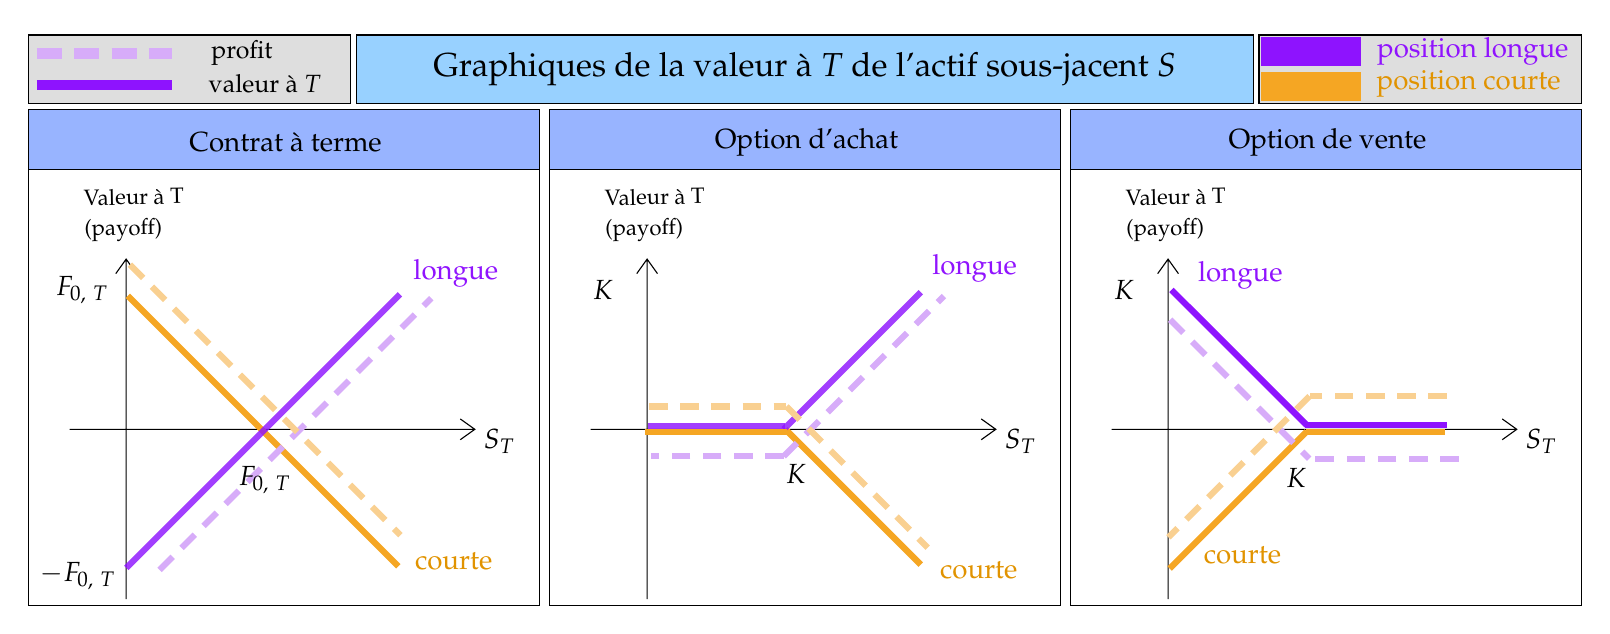
\begin{tikzpicture}[x=0.75pt,y=0.75pt,yscale=-1,xscale=1]
%uncomment if require: \path (0,533.3333282470703); %set diagram left start at 0, and has height of 533.3333282470703

%Shape: Rectangle [id:dp5014293673202075] 
\draw  [fill={rgb, 255:red, 152; green, 209; blue, 255 }  ,fill opacity=1 ] (185.17,2.33) -- (617.17,2.33) -- (617.17,35.33) -- (185.17,35.33) -- cycle ;
%Shape: Axis 2D [id:dp8910353553161174] 
\draw  (47,192.33) -- (242.17,192.33)(74.17,110.33) -- (74.17,274.17) (235.17,187.33) -- (242.17,192.33) -- (235.17,197.33) (69.17,117.33) -- (74.17,110.33) -- (79.17,117.33)  ;
%Straight Lines [id:da07902046514743155] 
\draw [color={rgb, 255:red, 245; green, 166; blue, 35 }  ,draw opacity=1 ][line width=2.25]    (75,128) -- (205.33,258.33) ;


%Straight Lines [id:da7529942024921858] 
\draw [color={rgb, 255:red, 142; green, 19; blue, 254 }  ,draw opacity=0.82 ][line width=2.25]    (74.25,259.08) -- (206.08,127.25) ;


%Shape: Rectangle [id:dp9569124985710353] 
\draw   (27,38.33) -- (273.17,38.33) -- (273.17,277.33) -- (27,277.33) -- cycle ;
%Shape: Rectangle [id:dp6038932286281922] 
\draw  [fill={rgb, 255:red, 152; green, 180; blue, 255 }  ,fill opacity=1 ] (27,38.33) -- (273.17,38.33) -- (273.17,67.13) -- (27,67.13) -- cycle ;
%Shape: Axis 2D [id:dp8487614270775223] 
\draw  (298,192.33) -- (493.17,192.33)(325.17,110.33) -- (325.17,274.17) (486.17,187.33) -- (493.17,192.33) -- (486.17,197.33) (320.17,117.33) -- (325.17,110.33) -- (330.17,117.33)  ;
%Straight Lines [id:da663442618971704] 
\draw [color={rgb, 255:red, 245; green, 166; blue, 35 }  ,draw opacity=1 ][line width=2.25]    (391.83,192.33) -- (457,257.5) ;


%Straight Lines [id:da8894317835492456] 
\draw [color={rgb, 255:red, 142; green, 19; blue, 254 }  ,draw opacity=0.82 ][line width=2.25]    (391,192.33) -- (457.08,126.25) ;


%Shape: Rectangle [id:dp8705141044857434] 
\draw   (278,38.33) -- (524.17,38.33) -- (524.17,277.33) -- (278,277.33) -- cycle ;
%Shape: Rectangle [id:dp12563706806770858] 
\draw  [fill={rgb, 255:red, 152; green, 180; blue, 255 }  ,fill opacity=1 ] (278,38.33) -- (524.17,38.33) -- (524.17,67.13) -- (278,67.13) -- cycle ;
%Straight Lines [id:da7370574620781261] 
\draw [color={rgb, 255:red, 142; green, 19; blue, 254 }  ,draw opacity=0.82 ][line width=2.25]    (325.54,190.62) -- (391.67,190.62) ;


%Straight Lines [id:da46421889356503176] 
\draw [color={rgb, 255:red, 245; green, 166; blue, 35 }  ,draw opacity=1 ][line width=2.25]    (324,193.62) -- (392.67,193.62) ;


%Shape: Axis 2D [id:dp12218006106251589] 
\draw  (549,192.33) -- (744.17,192.33)(576.17,110.33) -- (576.17,274.17) (737.17,187.33) -- (744.17,192.33) -- (737.17,197.33) (571.17,117.33) -- (576.17,110.33) -- (581.17,117.33)  ;
%Straight Lines [id:da05808191016293862] 
\draw [color={rgb, 255:red, 142; green, 19; blue, 254 }  ,draw opacity=1 ][line width=2.25]    (577.83,125.17) -- (643,190.33) ;


%Straight Lines [id:da6579640777364959] 
\draw [color={rgb, 255:red, 245; green, 166; blue, 35 }  ,draw opacity=1 ][line width=2.25]    (576.92,259.42) -- (643,193.33) ;


%Shape: Rectangle [id:dp6536765107760714] 
\draw   (529,38.33) -- (775.17,38.33) -- (775.17,277.33) -- (529,277.33) -- cycle ;
%Shape: Rectangle [id:dp8746319789223336] 
\draw  [fill={rgb, 255:red, 152; green, 180; blue, 255 }  ,fill opacity=1 ] (529,38.33) -- (775.17,38.33) -- (775.17,67.13) -- (529,67.13) -- cycle ;
%Straight Lines [id:da9314658151780497] 
\draw [color={rgb, 255:red, 245; green, 166; blue, 35 }  ,draw opacity=1 ][line width=2.25]    (709.67,193.62) -- (642.67,193.62) ;


%Straight Lines [id:da7353378001942827] 
\draw [color={rgb, 255:red, 142; green, 19; blue, 254 }  ,draw opacity=1 ][line width=2.25]    (642,190.33) -- (710.67,190.33) ;


%Straight Lines [id:da6447135481537327] 
\draw [color={rgb, 255:red, 215; green, 172; blue, 249 }  ,draw opacity=1 ][line width=2.25]  [dash pattern={on 6.75pt off 4.5pt}]  (90.25,260.08) -- (221.17,129.17) ;


%Straight Lines [id:da24025984300874126] 
\draw [color={rgb, 255:red, 215; green, 172; blue, 249 }  ,draw opacity=1 ][line width=2.25]  [dash pattern={on 6.75pt off 4.5pt}]  (391,205.33) -- (468.17,128.17) ;


%Straight Lines [id:da8831860343653457] 
\draw [color={rgb, 255:red, 215; green, 172; blue, 249 }  ,draw opacity=1 ][line width=2.25]  [dash pattern={on 6.75pt off 4.5pt}]  (391,205.33) -- (327.17,205.33) ;


%Straight Lines [id:da18639838701307276] 
\draw [color={rgb, 255:red, 215; green, 172; blue, 249 }  ,draw opacity=1 ][line width=2.25]  [dash pattern={on 6.75pt off 4.5pt}]  (577.17,139.5) -- (644.17,206.5) ;


%Straight Lines [id:da7126780450899792] 
\draw [color={rgb, 255:red, 215; green, 172; blue, 249 }  ,draw opacity=1 ][line width=2.25]  [dash pattern={on 6.75pt off 4.5pt}]  (716.17,206.5) -- (644.17,206.5) ;


%Straight Lines [id:da4974018498235153] 
\draw [color={rgb, 255:red, 249; green, 208; blue, 145 }  ,draw opacity=1 ][line width=2.25]  [dash pattern={on 6.75pt off 4.5pt}]  (76,113) -- (206.33,243.33) ;


%Straight Lines [id:da079381899397444] 
\draw [color={rgb, 255:red, 249; green, 208; blue, 145 }  ,draw opacity=1 ][line width=2.25]  [dash pattern={on 6.75pt off 4.5pt}]  (392.33,181.33) -- (460.33,249.33) ;


%Straight Lines [id:da6931960986042278] 
\draw [color={rgb, 255:red, 249; green, 208; blue, 145 }  ,draw opacity=1 ][line width=2.25]  [dash pattern={on 6.75pt off 4.5pt}]  (326.17,181.33) -- (392.33,181.33) ;


%Straight Lines [id:da13892219800463912] 
\draw [color={rgb, 255:red, 249; green, 208; blue, 145 }  ,draw opacity=1 ][line width=2.25]  [dash pattern={on 6.75pt off 4.5pt}]  (644.33,176.33) -- (576.33,244.33) ;


%Straight Lines [id:da8423794637164237] 
\draw [color={rgb, 255:red, 249; green, 208; blue, 145 }  ,draw opacity=1 ][line width=2.25]  [dash pattern={on 6.75pt off 4.5pt}]  (710.5,176.33) -- (644.33,176.33) ;


%Shape: Rectangle [id:dp6320359207595536] 
\draw  [fill={rgb, 255:red, 222; green, 222; blue, 222 }  ,fill opacity=1 ] (27,2.33) -- (182.17,2.33) -- (182.17,35.33) -- (27,35.33) -- cycle ;
%Straight Lines [id:da6914853181961316] 
\draw [color={rgb, 255:red, 215; green, 172; blue, 249 }  ,draw opacity=1 ][line width=3.75]  [dash pattern={on 9pt off 4.5pt}]  (31.17,11.33) -- (96.17,11.33) ;


%Straight Lines [id:da1620707780626105] 
\draw [color={rgb, 255:red, 142; green, 19; blue, 254 }  ,draw opacity=1 ][line width=3.75]    (31.17,26.33) -- (96.17,26.33) ;



%Shape: Rectangle [id:dp2381964955840581] 
\draw  [fill={rgb, 255:red, 222; green, 222; blue, 222 }  ,fill opacity=1 ] (620,2.33) -- (775.17,2.33) -- (775.17,35.33) -- (620,35.33) -- cycle ;
%Shape: Rectangle [id:dp2723528710393448] 
\draw  [draw opacity=0][fill={rgb, 255:red, 142; green, 19; blue, 254 }  ,fill opacity=1 ] (621,3.33) -- (669.17,3.33) -- (669.17,17.33) -- (621,17.33) -- cycle ;
%Shape: Rectangle [id:dp5738737247232852] 
\draw  [draw opacity=0][fill={rgb, 255:red, 245; green, 166; blue, 35 }  ,fill opacity=1 ] (621,20.33) -- (669.17,20.33) -- (669.17,34.33) -- (621,34.33) -- cycle ;

% Text Node
\draw (254,198) node   [align=left] {$\displaystyle S_{T}$};
% Text Node
\draw (53,125) node   [align=left] {$\displaystyle F_{0,\ T}$};
% Text Node
\draw (51,263) node   [align=left] {$\displaystyle -F_{0,\ T}$};
% Text Node
\draw (78,89) node  [font=\small,rotate=-358.99] [align=left] {{\footnotesize Valeur à T }\\{\footnotesize (payoff)}};
% Text Node
\draw (141,217) node   [align=left] {$\displaystyle F_{0,\ T}$};
% Text Node
\draw (151,54) node   [align=left] {Contrat à terme};
% Text Node
\draw (505,198) node   [align=left] {$\displaystyle S_{T}$};
% Text Node
\draw (304,125) node   [align=left] {$\displaystyle K$};
% Text Node
\draw (329,89) node  [font=\small,rotate=-358.99] [align=left] {{\footnotesize Valeur à T }\\{\footnotesize (payoff)}};
% Text Node
\draw (397,214) node   [align=left] {$\displaystyle K$};
% Text Node
\draw (401.17,18.83) node  [font=\large] [align=left] {Graphiques de la valeur à $\displaystyle T$ de l'actif sous-jacent $\displaystyle S$};
% Text Node
\draw (402,54) node   [align=left] {Option d'achat};
% Text Node
\draw (756,198) node   [align=left] {$\displaystyle S_{T}$};
% Text Node
\draw (555,125) node   [align=left] {$\displaystyle K$};
% Text Node
\draw (580,89) node  [font=\small,rotate=-358.99] [align=left] {{\footnotesize Valeur à T }\\{\footnotesize (payoff)}};
% Text Node
\draw (638,216) node   [align=left] {$\displaystyle K$};
% Text Node
\draw (611,118) node  [color={rgb, 255:red, 144; green, 19; blue, 254 }  ,opacity=1 ] [align=left] {longue};
% Text Node
\draw (612,253) node  [color={rgb, 255:red, 225; green, 147; blue, 0 }  ,opacity=1 ] [align=left] {courte};
% Text Node
\draw (653,54) node   [align=left] {Option de vente};
% Text Node
\draw (485,260) node  [color={rgb, 255:red, 225; green, 147; blue, 0 }  ,opacity=1 ] [align=left] {courte};
% Text Node
\draw (232,256) node  [color={rgb, 255:red, 225; green, 147; blue, 0 }  ,opacity=1 ] [align=left] {courte};
% Text Node
\draw (483,115) node  [color={rgb, 255:red, 144; green, 19; blue, 254 }  ,opacity=1 ] [align=left] {longue};
% Text Node
\draw (233,117) node  [color={rgb, 255:red, 144; green, 19; blue, 254 }  ,opacity=1 ] [align=left] {longue};
% Text Node
\draw (130,11) node  [font=\small] [align=left] {profit};
% Text Node
\draw (141,26) node  [font=\small] [align=left] {valeur à $\displaystyle T$};
% Text Node
\draw (723,10) node  [color={rgb, 255:red, 144; green, 19; blue, 254 }  ,opacity=1 ] [align=left] {position longue};
% Text Node
\draw (721,26) node  [color={rgb, 255:red, 225; green, 147; blue, 0 }  ,opacity=1 ] [align=left] {position courte};


\end{tikzpicture}
\end{center}

\newpage
\begin{multicols*}{2}

\section{Introduction aux Forwards et aux options}

\begin{distributions}[Terminologie]
\begin{description}
	\item[Premium] Flux financiers à $t = 0$;
	\item	Si \textcolor{blue}{positif}, il s'agît d'un \textbf{coût} ;
	\item	Si \textcolor{red}{négatif}, il s'agît d'une \textbf{compensation}.
	\item[Valeur à l'échéance $T$ (payoff):]	Les flux de trésorie au temps $t = T$;
	\item[Profit\footnote{\textbf{V}aleure \textbf{A}ccumulée au taux sans risque.}	] 
	\begin{align*}
	&=	\begin{cases}
			\text{Payoff} - VA(\text{Premium})&	\text{si position longue}	\\
			\text{Payoff} + VA(\text{Premium})	&	\text{si position courte}
		\end{cases} \\
	&\Leftrightarrow		VA(\text{flux de trésorie})
	\end{align*}
	\tcbline
	\item[$r_f$:] taux sans risque. 
	\item[]	Peut être exprimé comme une force d'intérêt $r$ continue ou comme un taux d'intérêt $r_{f}$.
\end{description}
\end{distributions}

\begin{definitionNOHFILL}[Contrat à terme]
Contrat selon lequel: 
\begin{itemize}
	\item	\textit{deux} partis s'\textbf{engagent} d'\textbf{échanger}---un à \textit{acheter} et l'autre à \textit{vendre};
	\item	une \textit{certaine} \textbf{quantité} d'un \textit{certain} \textbf{bien}---l'actif sous-jacent $S$;	
	\item	à un \textit{certain} \textbf{prix}---prix à terme $F_{0, T}$;
	\item	à un \textit{certain} \textbf{endroit} à une \textit{certaine} \textbf{date}---date d'échéance, $T$;
\end{itemize}

L'engagement est au départ à $t = 0$.

\begin{distributions}[Notation de prix]
%\begin{multicols*}{2}
\begin{itemize}
	\item[$S_{t}$:] \textbf{Prix du sous-jacent} à $t$ \textit{(\textbf{spot price})};
	\item[$S_{0}$:] \textbf{Prix au comptant};
	\item	Le prix au comptant représente le paiement pour la livraison immédiate à $t = 0$.
	\item[$F_{0, T}$:]	est le \textbf{prix à terme};
	\item	$F_{0, T} = S_{0} \textrm{e}^{r (T - 0)}$
	\item[$F_{0, 0}$:]	est nul;
	\item	La notation $F_{0, T}$ vient de \og future \fg{} ou \og forward \fg{}.
\end{itemize}
%\end{multicols*}
\end{distributions}

\begin{formula}{Exemple de bateau}
\begin{itemize}
	\item	Je veux acheter un \textit{(quantité)} bateau \textit{(bien)} mais ça m'est inconvénient de l'avoir maintenant;
	\item	En lieu, puisque je veux l'acheter maintenant, je signe une entente \textit{(engagement)} pour l'acheter;
	\item	La seule différence entre l'acheter aujourd'hui \textit{(au prix au comptant $S_{0}$)} et l'acheter lorsque la neige fond \textit{(au prix à terme $F_{0, T}$)} est l'accumulation d'intérêt;
	\item	Puisqu'on suppose tout les deux d'êtres fiables et sans risque, le prix est accumulé au taux sans risque ($r$) et le prix payable rendu à l'été ($T$) sera $F_{0, T} = S_{0} \textrm{e}^{r (T - 0)}$;
\end{itemize}
\end{formula}
\end{definitionNOHFILL}

\begin{definitionNOHFILL}[Exercice (levée)]
Décision d'\textit{exercer} l'option d'achat ou de vente.

\begin{distributions}[Notation]
\begin{itemize}
	\item[$K$:]	\textbf{Prix d'exercice} \textit{(\textbf{strike price})};
\end{itemize}
\end{distributions}

\begin{conceptgen}{Types d'exercices}
\begin{description}
	\item[\textbf{\underline{E}}uropéen:]		\textbf{Au moment} d'\textbf{\underline{e}}xpiration de l'option $T$;
	\item[\textbf{\underline{A}}méricain:]	\textbf{N'importe quand} (\textbf{\underline{a}}ny moment) d'ici $T$;
	\item[\textbf{\underline{B}}ermudien:]	À \textbf{quelques périodes} (\textbf{\underline{b}}ounded periods) d'ici $T$;
\end{description}
En réalité, la \textit{majorité sont américain}  et donc nous effectuons uniquement des calculs avec ce type.
\end{conceptgen}
\end{definitionNOHFILL}

\begin{definitionNOHFILL}[Option d'achat]
Contrat qui: 
\begin{itemize}
	\item	\textit{permet} \textbf{(optionnel)} à son \textit{détenteur} d'\textbf{acheter};
	\item	une \textit{certaine} \textbf{quantité} d'un \textit{certain} \textbf{bien}---l'actif sous-jacent;	
	\item	à un \textit{certain} \textbf{prix}---prix d'exercice $K$;
	\item	à un \textit{certain} \textbf{endroit} à, ou d'ici, une \textit{certaine} \textbf{date}---date d'échéance, $T$;
\end{itemize}

%\textbf{Notation de prix}:
%\begin{multicols*}{2}
%\begin{itemize}
%	\item[$C_{t}$:] 
%	\item[$C_{0}$:] 
%\end{itemize}
%\end{multicols*}
\end{definitionNOHFILL}

\begin{definitionNOHFILL}[Option de vente]
Contrat qui \textit{permet} à son \textit{détenteur} de \textbf{vendre} au lieu d'acheter.
\end{definitionNOHFILL}


\paragraph{Quelques définitions}
\begin{description}
\item[$F_{0,T}$] Prix \textit{forward} du sous-jacent au temps $T$, qu'on définit comme
\[F_{0,T} = S_0 (1 + r_f)^{T}\]
\item[$F_{0,T}^{P}$] Prix d'un forward prépayé, i.e. on débourse $F_{0,T}^{P}$ à $t=0$ et on reçoit le sous-jacent à $t  = T$, alors
\[F_{0,T}^{P} = F_{0,T} (1 + r_f)^{-T}\]
\end{description}

\paragraph{Achat ferme et emprunt} On utilise parfois la lettre $S$ pour désigner dans stratégie l'action de faire un achat ferme (i.e. acheter et se faire livrer le sous-jacent à $t=0$) et $B$ pour désigner un dépôt/emprunt (qu'on exprime comme une obligation zéro-coupon).


\subsection*{$Call(K,T)$}
Contrat qui \textit{permet} au détenteur de se procurer $S$ au prix $K$ à l'échéance $T$. \textbf{position longue dans le sous-jacent}
\[Premium = C(K,T) \]

\subsection*{$Put(K,T)$}
Contrat qui \textit{permet} au détenteur de vendre $S$ au prix $K$ à l'échéance $T$. \textbf{position courte dans le sous-jacent}
\[Premium = P(K,T)\]

\subsection*{Forward synthétique}
On peut créer un Forward synthétique 2 de façon (en combinant d'autres transactions) : 
\[Forward = Stock - Bond \]
\[Forward = Call(K,T) - Put(K,T) \]
Ces deux égalités définissent la \emph{Put-Call Parity} vu un peu plus loin.


\section{Stratégie de couverture}
\subsection*{Floor}
On achète $S$ en se protégant contre une baisse trop importante du sous-jacent (\textbf{position longue})
\[Floor = Stock + Put(K,T)\]
\[Premium = S_0 + P(K,T) > 0\]
\[Payoff = 
\begin{cases}
K					& , S_T \leq K \\
S_T				& , S_T > K \\
\end{cases}
\]


\tikzset{every picture/.style={line width=0.75pt}} %set default line width to 0.75pt        

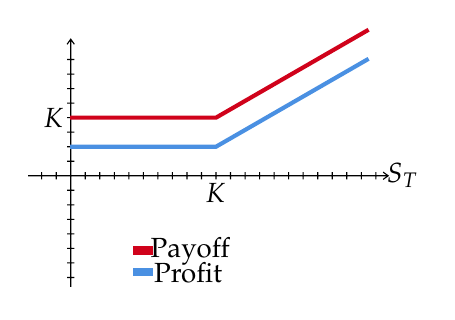
\begin{tikzpicture}[x=0.75pt,y=0.75pt,yscale=-0.35,xscale=0.35]
%uncomment if require: \path (0,363); %set diagram left start at 0, and has height of 363

%Shape: Axis 2D [id:dp5284616222676404] 
\draw  (14,196) -- (509.5,196)(72.5,8) -- (72.5,349) (502.5,191) -- (509.5,196) -- (502.5,201) (67.5,15) -- (72.5,8) -- (77.5,15) (92.5,191) -- (92.5,201)(112.5,191) -- (112.5,201)(132.5,191) -- (132.5,201)(152.5,191) -- (152.5,201)(172.5,191) -- (172.5,201)(192.5,191) -- (192.5,201)(212.5,191) -- (212.5,201)(232.5,191) -- (232.5,201)(252.5,191) -- (252.5,201)(272.5,191) -- (272.5,201)(292.5,191) -- (292.5,201)(312.5,191) -- (312.5,201)(332.5,191) -- (332.5,201)(352.5,191) -- (352.5,201)(372.5,191) -- (372.5,201)(392.5,191) -- (392.5,201)(412.5,191) -- (412.5,201)(432.5,191) -- (432.5,201)(452.5,191) -- (452.5,201)(472.5,191) -- (472.5,201)(492.5,191) -- (492.5,201)(52.5,191) -- (52.5,201)(32.5,191) -- (32.5,201)(67.5,176) -- (77.5,176)(67.5,156) -- (77.5,156)(67.5,136) -- (77.5,136)(67.5,116) -- (77.5,116)(67.5,96) -- (77.5,96)(67.5,76) -- (77.5,76)(67.5,56) -- (77.5,56)(67.5,36) -- (77.5,36)(67.5,216) -- (77.5,216)(67.5,236) -- (77.5,236)(67.5,256) -- (77.5,256)(67.5,276) -- (77.5,276)(67.5,296) -- (77.5,296)(67.5,316) -- (77.5,316)(67.5,336) -- (77.5,336) ;
\draw   ;
%Straight Lines [id:da07170428809155915] 
\draw [color={rgb, 255:red, 208; green, 2; blue, 27 }  ,draw opacity=1 ][line width=1.5]    (71.5,116) -- (272.5,116) -- (482.5,-5) ;


%Straight Lines [id:da9437345853796594] 
\draw [color={rgb, 255:red, 74; green, 144; blue, 226 }  ,draw opacity=1 ][line width=1.5]    (71.5,156) -- (272.5,156) -- (482.5,35) ;


%Straight Lines [id:da10527715337594734] 
\draw [color={rgb, 255:red, 208; green, 2; blue, 27 }  ,draw opacity=1 ][line width=3]    (158.5,299) -- (185.5,299) ;


%Straight Lines [id:da20667043631469095] 
\draw [color={rgb, 255:red, 74; green, 144; blue, 226 }  ,draw opacity=1 ][line width=3]    (158.5,328) -- (185.5,328) ;




% Text Node
\draw (529,196) node  [align=left] {$\displaystyle S_{T}$};
% Text Node
\draw (272,220) node   {$K$};
% Text Node
\draw (237,300) node  [align=left] {Payoff};
% Text Node
\draw (234,329) node  [align=left] {Profit};
% Text Node
\draw (49,117) node   {$K$};


\end{tikzpicture}



\subsection*{Cap}
On vend à découvert $S$ en se protégant contre une hausse trop importante du sous-jacent (car il faudra éventuellement le racheter!). \textbf{Position courte}.
\[Cap = Call(K,T) - Stock\]
\[Premium = C(K,T) - S_0 < 0\]
\[Payoff
\begin{cases}
- S_T 			& , S_T \leq K \\
- K				& , S_T > K \\
\end{cases}
\]


\tikzset{every picture/.style={line width=0.75pt}} %set default line width to 0.75pt        

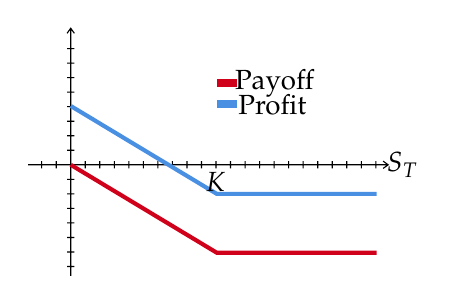
\begin{tikzpicture}[x=0.75pt,y=0.75pt,yscale=-0.35,xscale=0.35]
%uncomment if require: \path (0,363); %set diagram left start at 0, and has height of 363

%Shape: Axis 2D [id:dp037268718196239004] 
\draw  (14,196) -- (509.5,196)(72.5,8) -- (72.5,349) (502.5,191) -- (509.5,196) -- (502.5,201) (67.5,15) -- (72.5,8) -- (77.5,15) (92.5,191) -- (92.5,201)(112.5,191) -- (112.5,201)(132.5,191) -- (132.5,201)(152.5,191) -- (152.5,201)(172.5,191) -- (172.5,201)(192.5,191) -- (192.5,201)(212.5,191) -- (212.5,201)(232.5,191) -- (232.5,201)(252.5,191) -- (252.5,201)(272.5,191) -- (272.5,201)(292.5,191) -- (292.5,201)(312.5,191) -- (312.5,201)(332.5,191) -- (332.5,201)(352.5,191) -- (352.5,201)(372.5,191) -- (372.5,201)(392.5,191) -- (392.5,201)(412.5,191) -- (412.5,201)(432.5,191) -- (432.5,201)(452.5,191) -- (452.5,201)(472.5,191) -- (472.5,201)(492.5,191) -- (492.5,201)(52.5,191) -- (52.5,201)(32.5,191) -- (32.5,201)(67.5,176) -- (77.5,176)(67.5,156) -- (77.5,156)(67.5,136) -- (77.5,136)(67.5,116) -- (77.5,116)(67.5,96) -- (77.5,96)(67.5,76) -- (77.5,76)(67.5,56) -- (77.5,56)(67.5,36) -- (77.5,36)(67.5,216) -- (77.5,216)(67.5,236) -- (77.5,236)(67.5,256) -- (77.5,256)(67.5,276) -- (77.5,276)(67.5,296) -- (77.5,296)(67.5,316) -- (77.5,316)(67.5,336) -- (77.5,336) ;
\draw   ;
%Straight Lines [id:da3847211306528634] 
\draw [color={rgb, 255:red, 208; green, 2; blue, 27 }  ,draw opacity=1 ][line width=1.5]    (72.5,196) -- (273.5,317) -- (493.5,317) ;


%Straight Lines [id:da10620263985508471] 
\draw [color={rgb, 255:red, 208; green, 2; blue, 27 }  ,draw opacity=1 ][line width=3]    (274.5,83) -- (301.5,83) ;


%Straight Lines [id:da0036212401211522804] 
\draw [color={rgb, 255:red, 74; green, 144; blue, 226 }  ,draw opacity=1 ][line width=3]    (274.5,112) -- (301.5,112) ;



%Straight Lines [id:da011019730384494886] 
\draw [color={rgb, 255:red, 74; green, 144; blue, 226 }  ,draw opacity=1 ][line width=1.5]    (72.5,115) -- (273.5,236) -- (493.5,236) ;



% Text Node
\draw (529,196) node  [align=left] {$\displaystyle S_{T}$};
% Text Node
\draw (353,84) node  [align=left] {Payoff};
% Text Node
\draw (350,113) node  [align=left] {Profit};
% Text Node
\draw (272,220) node   {$K$};


\end{tikzpicture}



\subsection*{Bull Spread}
Combinaison de 2 Call (ou 2 Put) pour spéculer sur un marché haussier. Avec $K_1 < K_2$, on a
\paragraph{Avec option d'achat}
\[Bull Spread (Call) = Call(K_1, T) - Call(K_2, T) \]

\[Premium = C(K_1, T) - Call(K_2, T) > 0 \]
\[Payoff = 
\begin{cases}
0					& , S_T \leq K_1 \\
S_T - K_1		& , k_1 < S_T \leq K_2 \\
K_2 -K_1		& , S_T > K_2 \\
\end{cases}
\]
\paragraph{Avec option de vente}
\[Bull Spread(Put) = Put(K_1, T) - Put(K_2,T) \]
\[Premium = P(K_1,T) - P(K_2, T) < 0\]
\[Payoff = 
\begin{cases}
K_1 - K_2 			& , S_T \leq K_1 \\
K_2 - S_T				& , K_1 < S_T \leq K_2 \\
0							& , S_T > K_2 \\
\end{cases}
\]



\tikzset{every picture/.style={line width=0.75pt}} %set default line width to 0.75pt        

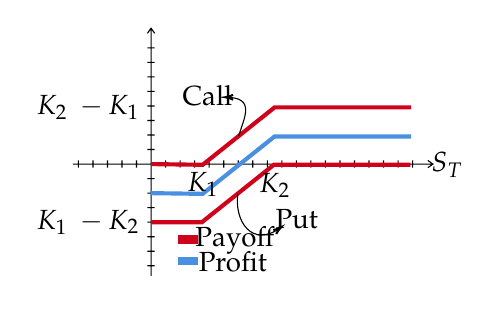
\begin{tikzpicture}[x=0.75pt,y=0.75pt,yscale=-0.35,xscale=0.35]
%uncomment if require: \path (0,363); %set diagram left start at 0, and has height of 363

%Shape: Axis 2D [id:dp28449288707577314] 
\draw  (14,195) -- (509.5,195)(121.5,8) -- (121.5,349) (502.5,190) -- (509.5,195) -- (502.5,200) (116.5,15) -- (121.5,8) -- (126.5,15) (141.5,190) -- (141.5,200)(161.5,190) -- (161.5,200)(181.5,190) -- (181.5,200)(201.5,190) -- (201.5,200)(221.5,190) -- (221.5,200)(241.5,190) -- (241.5,200)(261.5,190) -- (261.5,200)(281.5,190) -- (281.5,200)(301.5,190) -- (301.5,200)(321.5,190) -- (321.5,200)(341.5,190) -- (341.5,200)(361.5,190) -- (361.5,200)(381.5,190) -- (381.5,200)(401.5,190) -- (401.5,200)(421.5,190) -- (421.5,200)(441.5,190) -- (441.5,200)(461.5,190) -- (461.5,200)(481.5,190) -- (481.5,200)(101.5,190) -- (101.5,200)(81.5,190) -- (81.5,200)(61.5,190) -- (61.5,200)(41.5,190) -- (41.5,200)(21.5,190) -- (21.5,200)(116.5,175) -- (126.5,175)(116.5,155) -- (126.5,155)(116.5,135) -- (126.5,135)(116.5,115) -- (126.5,115)(116.5,95) -- (126.5,95)(116.5,75) -- (126.5,75)(116.5,55) -- (126.5,55)(116.5,35) -- (126.5,35)(116.5,215) -- (126.5,215)(116.5,235) -- (126.5,235)(116.5,255) -- (126.5,255)(116.5,275) -- (126.5,275)(116.5,295) -- (126.5,295)(116.5,315) -- (126.5,315)(116.5,335) -- (126.5,335) ;
\draw   ;
%Straight Lines [id:da9209384368986784] 
\draw [color={rgb, 255:red, 208; green, 2; blue, 27 }  ,draw opacity=1 ][line width=1.5]    (121.5,195) -- (192.5,196) -- (291.5,117) -- (479.5,117) ;


%Straight Lines [id:da37977537439547226] 
\draw [color={rgb, 255:red, 208; green, 2; blue, 27 }  ,draw opacity=1 ][line width=3]    (158.5,299) -- (185.5,299) ;


%Straight Lines [id:da9460733927110921] 
\draw [color={rgb, 255:red, 74; green, 144; blue, 226 }  ,draw opacity=1 ][line width=3]    (158.5,328) -- (185.5,328) ;



%Straight Lines [id:da9014316388237789] 
\draw [color={rgb, 255:red, 74; green, 144; blue, 226 }  ,draw opacity=1 ][line width=1.5]    (120.5,235) -- (192.5,236) -- (291.5,157) -- (479.5,157) ;


%Straight Lines [id:da22160788848594903] 
\draw [color={rgb, 255:red, 208; green, 2; blue, 27 }  ,draw opacity=1 ][line width=1.5]    (121.5,275) -- (191.5,275) -- (290.5,196) -- (478.5,196) ;


%Curve Lines [id:da09447744102237843] 
\draw    (241,235.5) .. controls (235.56,272.63) and (260,311.22) .. (299.3,282.88) ;
\draw [shift={(300.5,282)}, rotate = 503.13] [color={rgb, 255:red, 0; green, 0; blue, 0 }  ][line width=0.75]    (10.93,-3.29) .. controls (6.95,-1.4) and (3.31,-0.3) .. (0,0) .. controls (3.31,0.3) and (6.95,1.4) .. (10.93,3.29)   ;

%Curve Lines [id:da08283708021002456] 
\draw    (242,156.5) .. controls (250.37,129.41) and (265.05,103.78) .. (225.35,103.02) ;
\draw [shift={(223.5,103)}, rotate = 360] [color={rgb, 255:red, 0; green, 0; blue, 0 }  ][line width=0.75]    (10.93,-3.29) .. controls (6.95,-1.4) and (3.31,-0.3) .. (0,0) .. controls (3.31,0.3) and (6.95,1.4) .. (10.93,3.29)   ;


% Text Node
\draw (529,196) node  [align=left] {$\displaystyle S_{T}$};
% Text Node
\draw (193,223) node   {$K_{1}$};
% Text Node
\draw (237,300) node  [align=left] {Payoff};
% Text Node
\draw (234,329) node  [align=left] {Profit};
% Text Node
\draw (35,117) node   {$K_{2} \ -K_{1}$};
% Text Node
\draw (292,224) node   {$K_{2}$};
% Text Node
\draw (322,271) node  [align=left] {Put};
% Text Node
\draw (199,101) node  [align=left] {Call};
% Text Node
\draw (35,275) node   {$K_{1} \ -K_{2}$};


\end{tikzpicture}




\subsection*{Bear Spread}
Combinaison de 2 Call ou 2 Put pour spéculer sur un marché baissier.
\paragraph{Avec option d'achat}
\begin{align*}
Bear(Call) & =  - Bull(Call) \\
& = Call(K_2, T) - Call(K_1, T) \\
Premium		& = 	 C(K_2,T) - C(K_1,T) < 0 \\
Profit	& = 
\begin{cases}
0					& , S_T \leq K_1 \\
K_1 - S_T 	& , K_1 < S_T \leq K_2 \\
-(K_2 - K_1)& , S_T > K_2 \\
\end{cases}
\end{align*}

\paragraph{Avec option de vente}
\begin{align*}
Bear(Put) 				& =  - Bull(Put) \\
								& = Put(K_2, T) - Put(K_1, T) \\
Premium					& = 	 P(K_2,T) - P(K_1,T) > 0 \\
Profit						& = 
\begin{cases}
K_2 - K_1					& , S_T \leq K_1 \\
K_2 - S_T 				& , K_1 < S_T \leq K_2 \\
0								& , S_T > K_2 \\
\end{cases}
\end{align*}


\tikzset{every picture/.style={line width=0.75pt}} %set default line width to 0.75pt        

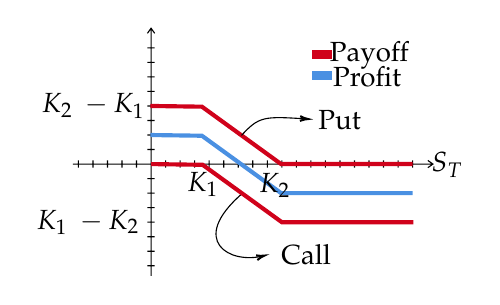
\begin{tikzpicture}[x=0.75pt,y=0.75pt,yscale=-0.35,xscale=0.35]
%uncomment if require: \path (0,363); %set diagram left start at 0, and has height of 363

%Shape: Axis 2D [id:dp5006858190484493] 
\draw  (14,195) -- (509.5,195)(121.5,8) -- (121.5,349) (502.5,190) -- (509.5,195) -- (502.5,200) (116.5,15) -- (121.5,8) -- (126.5,15) (141.5,190) -- (141.5,200)(161.5,190) -- (161.5,200)(181.5,190) -- (181.5,200)(201.5,190) -- (201.5,200)(221.5,190) -- (221.5,200)(241.5,190) -- (241.5,200)(261.5,190) -- (261.5,200)(281.5,190) -- (281.5,200)(301.5,190) -- (301.5,200)(321.5,190) -- (321.5,200)(341.5,190) -- (341.5,200)(361.5,190) -- (361.5,200)(381.5,190) -- (381.5,200)(401.5,190) -- (401.5,200)(421.5,190) -- (421.5,200)(441.5,190) -- (441.5,200)(461.5,190) -- (461.5,200)(481.5,190) -- (481.5,200)(101.5,190) -- (101.5,200)(81.5,190) -- (81.5,200)(61.5,190) -- (61.5,200)(41.5,190) -- (41.5,200)(21.5,190) -- (21.5,200)(116.5,175) -- (126.5,175)(116.5,155) -- (126.5,155)(116.5,135) -- (126.5,135)(116.5,115) -- (126.5,115)(116.5,95) -- (126.5,95)(116.5,75) -- (126.5,75)(116.5,55) -- (126.5,55)(116.5,35) -- (126.5,35)(116.5,215) -- (126.5,215)(116.5,235) -- (126.5,235)(116.5,255) -- (126.5,255)(116.5,275) -- (126.5,275)(116.5,295) -- (126.5,295)(116.5,315) -- (126.5,315)(116.5,335) -- (126.5,335) ;
\draw   ;
%Straight Lines [id:da13258465142858888] 
\draw [color={rgb, 255:red, 208; green, 2; blue, 27 }  ,draw opacity=1 ][line width=1.5]    (120.5,115) -- (191.5,116) -- (300.5,195) -- (481.5,195) ;


%Straight Lines [id:da7932939446362234] 
\draw [color={rgb, 255:red, 208; green, 2; blue, 27 }  ,draw opacity=1 ][line width=3]    (343.5,44) -- (370.5,44) ;


%Straight Lines [id:da14367852228745004] 
\draw [color={rgb, 255:red, 74; green, 144; blue, 226 }  ,draw opacity=1 ][line width=3]    (343.5,73) -- (370.5,73) ;



%Curve Lines [id:da6986177249173428] 
\draw    (246,155.5) .. controls (270.26,129.26) and (276.38,129) .. (335.69,132.88) ;
\draw [shift={(337.5,133)}, rotate = 183.75] [color={rgb, 255:red, 0; green, 0; blue, 0 }  ][line width=0.75]    (10.93,-3.29) .. controls (6.95,-1.4) and (3.31,-0.3) .. (0,0) .. controls (3.31,0.3) and (6.95,1.4) .. (10.93,3.29)   ;

%Curve Lines [id:da16730216097312656] 
\draw    (247,235.5) .. controls (172.25,300.35) and (229.33,333.34) .. (276.09,321.38) ;
\draw [shift={(277.5,321)}, rotate = 524.54] [color={rgb, 255:red, 0; green, 0; blue, 0 }  ][line width=0.75]    (10.93,-3.29) .. controls (6.95,-1.4) and (3.31,-0.3) .. (0,0) .. controls (3.31,0.3) and (6.95,1.4) .. (10.93,3.29)   ;

%Straight Lines [id:da38075245439918526] 
\draw [color={rgb, 255:red, 74; green, 144; blue, 226 }  ,draw opacity=1 ][line width=1.5]    (120.5,155) -- (191.5,156) -- (300.5,235) -- (481.5,235) ;


%Straight Lines [id:da001223510828637031] 
\draw [color={rgb, 255:red, 208; green, 2; blue, 27 }  ,draw opacity=1 ][line width=1.5]    (121.5,195) -- (192.5,196) -- (301.5,275) -- (482.5,275) ;



% Text Node
\draw (529,196) node  [align=left] {$\displaystyle S_{T}$};
% Text Node
\draw (193,223) node   {$K_{1}$};
% Text Node
\draw (422,45) node  [align=left] {Payoff};
% Text Node
\draw (419,74) node  [align=left] {Profit};
% Text Node
\draw (42,115) node   {$K_{2} \ -K_{1}$};
% Text Node
\draw (292,224) node   {$K_{2}$};
% Text Node
\draw (381,134) node  [align=left] {Put};
% Text Node
\draw (335,320) node  [align=left] {Call};
% Text Node
\draw (35,275) node   {$K_{1} \ -K_{2}$};


\end{tikzpicture}



\subsection*{Ratio Spread}
Cette stratégie est une combinaison un peu sur mesure (on ne peut pas nécessairement dire si elle est longue ou courte). On achète $n$ options d'achat à un prix d'exercice $K_1$ et on en vend $m$ à un prix d'exercice $K_2$.\footnote{On peut faire cette stratégie avec des options de vente aussi.}
\begin{align*}
Ratio Spread 		& 	= n Call(K_1, T) - m Call(K_2, T) \\
Premium				& = n C(K_1, T) - m C(K_2,T) \\
Payoff					& = ...
\end{align*}

\subsection*{Box Spread}
Cette stratégie réplique l'achat d'une obligation zéro-coupon, en impliquant 2 option d'achat et 2 options de vente.
\begin{align*}
Box Spread			& = Bull(Call) + Bear(Put) \\
& = Call(K_1, T) - Call(K_2, T)  \\
& + Put(K_2, T) - Put(K_1, T) \\
Premium				& = C(K_1, T) - C(K_2, T) \\
							&  + P(K_2, T) - P(K_1,T) >  0 \\
Payoff					& = K_2 - K_1  \ , \forall S_T \\
\end{align*}


\tikzset{every picture/.style={line width=0.75pt}} %set default line width to 0.75pt        

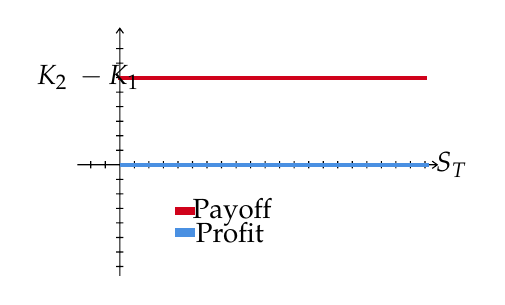
\begin{tikzpicture}[x=0.75pt,y=0.75pt,yscale=-0.35,xscale=0.35]
%uncomment if require: \path (0,363); %set diagram left start at 0, and has height of 363

%Shape: Axis 2D [id:dp6247716683220562] 
\draw  (14,196) -- (509.5,196)(72.5,8) -- (72.5,349) (502.5,191) -- (509.5,196) -- (502.5,201) (67.5,15) -- (72.5,8) -- (77.5,15) (92.5,191) -- (92.5,201)(112.5,191) -- (112.5,201)(132.5,191) -- (132.5,201)(152.5,191) -- (152.5,201)(172.5,191) -- (172.5,201)(192.5,191) -- (192.5,201)(212.5,191) -- (212.5,201)(232.5,191) -- (232.5,201)(252.5,191) -- (252.5,201)(272.5,191) -- (272.5,201)(292.5,191) -- (292.5,201)(312.5,191) -- (312.5,201)(332.5,191) -- (332.5,201)(352.5,191) -- (352.5,201)(372.5,191) -- (372.5,201)(392.5,191) -- (392.5,201)(412.5,191) -- (412.5,201)(432.5,191) -- (432.5,201)(452.5,191) -- (452.5,201)(472.5,191) -- (472.5,201)(492.5,191) -- (492.5,201)(52.5,191) -- (52.5,201)(32.5,191) -- (32.5,201)(67.5,176) -- (77.5,176)(67.5,156) -- (77.5,156)(67.5,136) -- (77.5,136)(67.5,116) -- (77.5,116)(67.5,96) -- (77.5,96)(67.5,76) -- (77.5,76)(67.5,56) -- (77.5,56)(67.5,36) -- (77.5,36)(67.5,216) -- (77.5,216)(67.5,236) -- (77.5,236)(67.5,256) -- (77.5,256)(67.5,276) -- (77.5,276)(67.5,296) -- (77.5,296)(67.5,316) -- (77.5,316)(67.5,336) -- (77.5,336) ;
\draw   ;
%Straight Lines [id:da015831328429750546] 
\draw [color={rgb, 255:red, 208; green, 2; blue, 27 }  ,draw opacity=1 ][line width=3]    (148.5,260) -- (175.5,260) ;


%Straight Lines [id:da9141937301503729] 
\draw [color={rgb, 255:red, 74; green, 144; blue, 226 }  ,draw opacity=1 ][line width=3]    (148.5,289) -- (175.5,289) ;



%Straight Lines [id:da6721376585792007] 
\draw [color={rgb, 255:red, 208; green, 2; blue, 27 }  ,draw opacity=1 ][line width=1.5]    (70.5,76) -- (495.5,76) ;


%Straight Lines [id:da647166999440681] 
\draw [color={rgb, 255:red, 74; green, 144; blue, 226 }  ,draw opacity=1 ][line width=1.5]    (72.5,196) -- (497.5,196) ;



% Text Node
\draw (529,196) node  [align=left] {$\displaystyle S_{T}$};
% Text Node
\draw (227,261) node  [align=left] {Payoff};
% Text Node
\draw (224,290) node  [align=left] {Profit};
% Text Node
\draw (29,76) node   {$K_{2} \ -K_{1}$};


\end{tikzpicture}




\subsection*{Collar}
La prime initiale du Collar peut être soit positive ou négative (dépendant du strike price).
\begin{align*}
Collar				& = Put(K_1, T) - Call(K_2, T) \\
Premium			& = P(K_1, T) - C(K_2,T) \\
Payoff				& = 
\begin{cases}
K_1 - S_T			& , S_T \leq K_1 \\
0						& , K_1 < S_T \leq K_2 \\
K_2 - S_T			& , S_T > K_2 \\
\end{cases}
\end{align*}


\tikzset{every picture/.style={line width=0.75pt}} %set default line width to 0.75pt        

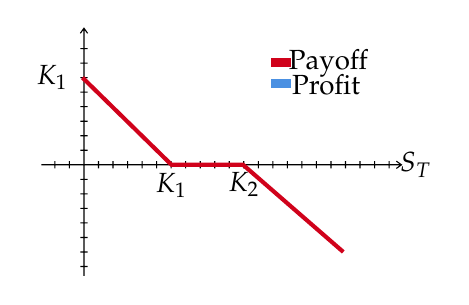
\begin{tikzpicture}[x=0.75pt,y=0.75pt,yscale=-0.35,xscale=0.35]
%uncomment if require: \path (0,363); %set diagram left start at 0, and has height of 363

%Shape: Axis 2D [id:dp6247716683220562] 
\draw  (14,196) -- (509.5,196)(72.5,8) -- (72.5,349) (502.5,191) -- (509.5,196) -- (502.5,201) (67.5,15) -- (72.5,8) -- (77.5,15) (92.5,191) -- (92.5,201)(112.5,191) -- (112.5,201)(132.5,191) -- (132.5,201)(152.5,191) -- (152.5,201)(172.5,191) -- (172.5,201)(192.5,191) -- (192.5,201)(212.5,191) -- (212.5,201)(232.5,191) -- (232.5,201)(252.5,191) -- (252.5,201)(272.5,191) -- (272.5,201)(292.5,191) -- (292.5,201)(312.5,191) -- (312.5,201)(332.5,191) -- (332.5,201)(352.5,191) -- (352.5,201)(372.5,191) -- (372.5,201)(392.5,191) -- (392.5,201)(412.5,191) -- (412.5,201)(432.5,191) -- (432.5,201)(452.5,191) -- (452.5,201)(472.5,191) -- (472.5,201)(492.5,191) -- (492.5,201)(52.5,191) -- (52.5,201)(32.5,191) -- (32.5,201)(67.5,176) -- (77.5,176)(67.5,156) -- (77.5,156)(67.5,136) -- (77.5,136)(67.5,116) -- (77.5,116)(67.5,96) -- (77.5,96)(67.5,76) -- (77.5,76)(67.5,56) -- (77.5,56)(67.5,36) -- (77.5,36)(67.5,216) -- (77.5,216)(67.5,236) -- (77.5,236)(67.5,256) -- (77.5,256)(67.5,276) -- (77.5,276)(67.5,296) -- (77.5,296)(67.5,316) -- (77.5,316)(67.5,336) -- (77.5,336) ;
\draw   ;
%Straight Lines [id:da015831328429750546] 
\draw [color={rgb, 255:red, 208; green, 2; blue, 27 }  ,draw opacity=1 ][line width=3]    (330.5,55) -- (357.5,55) ;


%Straight Lines [id:da9141937301503729] 
\draw [color={rgb, 255:red, 74; green, 144; blue, 226 }  ,draw opacity=1 ][line width=3]    (330.5,84) -- (357.5,84) ;



%Straight Lines [id:da6721376585792007] 
\draw [color={rgb, 255:red, 208; green, 2; blue, 27 }  ,draw opacity=1 ][line width=1.5]    (70.5,76) -- (193,196) -- (291.5,196) -- (429.5,316) ;



% Text Node
\draw (529,196) node  [align=left] {$\displaystyle S_{T}$};
% Text Node
\draw (409,56) node  [align=left] {Payoff};
% Text Node
\draw (406,85) node  [align=left] {Profit};
% Text Node
\draw (29,76) node   {$K_{1}$};
% Text Node
\draw (193,225) node   {$K_{1}$};
% Text Node
\draw (293,223) node   {$K_{2}$};


\end{tikzpicture}




\subsection*{Stock Covered by Collar}
\begin{itemize}
\item On effectue la même stratégie qu'un Collar, en ayant initialement le sous-jacent $S$. \textbf{Position longue dans le sous-jacent}.
\item Cette stratégie reproduit les flux monétaires d'un Bull Spread, alors
\end{itemize}
\begin{align*}
BullSpread				& = Collar + Stock \\
								& = Put(K_1, T) - Call(K_2, T) + Stock \\
Premium					& = P(K_1, T) - C(K_2,T) + S_0 > 0  \\
Payoff						& = 
\begin{cases}
K_1 					& , S_T \leq K_1 \\
S_T					& , K_1 < S_T \leq K_2 \\
K_2 					& , S_T > K_2 \\
\end{cases}
\end{align*}


\tikzset{every picture/.style={line width=0.75pt}} %set default line width to 0.75pt        

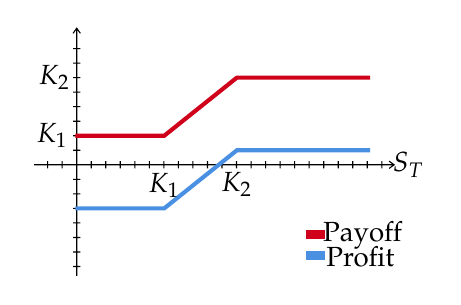
\begin{tikzpicture}[x=0.75pt,y=0.75pt,yscale=-0.35,xscale=0.35]
%uncomment if require: \path (0,363); %set diagram left start at 0, and has height of 363

%Shape: Axis 2D [id:dp20088335764830656] 
\draw  (14,196) -- (509.5,196)(72.5,8) -- (72.5,349) (502.5,191) -- (509.5,196) -- (502.5,201) (67.5,15) -- (72.5,8) -- (77.5,15) (92.5,191) -- (92.5,201)(112.5,191) -- (112.5,201)(132.5,191) -- (132.5,201)(152.5,191) -- (152.5,201)(172.5,191) -- (172.5,201)(192.5,191) -- (192.5,201)(212.5,191) -- (212.5,201)(232.5,191) -- (232.5,201)(252.5,191) -- (252.5,201)(272.5,191) -- (272.5,201)(292.5,191) -- (292.5,201)(312.5,191) -- (312.5,201)(332.5,191) -- (332.5,201)(352.5,191) -- (352.5,201)(372.5,191) -- (372.5,201)(392.5,191) -- (392.5,201)(412.5,191) -- (412.5,201)(432.5,191) -- (432.5,201)(452.5,191) -- (452.5,201)(472.5,191) -- (472.5,201)(492.5,191) -- (492.5,201)(52.5,191) -- (52.5,201)(32.5,191) -- (32.5,201)(67.5,176) -- (77.5,176)(67.5,156) -- (77.5,156)(67.5,136) -- (77.5,136)(67.5,116) -- (77.5,116)(67.5,96) -- (77.5,96)(67.5,76) -- (77.5,76)(67.5,56) -- (77.5,56)(67.5,36) -- (77.5,36)(67.5,216) -- (77.5,216)(67.5,236) -- (77.5,236)(67.5,256) -- (77.5,256)(67.5,276) -- (77.5,276)(67.5,296) -- (77.5,296)(67.5,316) -- (77.5,316)(67.5,336) -- (77.5,336) ;
\draw   ;
%Straight Lines [id:da10536374065219245] 
\draw [color={rgb, 255:red, 208; green, 2; blue, 27 }  ,draw opacity=1 ][line width=3]    (387.5,292) -- (414.5,292) ;


%Straight Lines [id:da016662989001628326] 
\draw [color={rgb, 255:red, 74; green, 144; blue, 226 }  ,draw opacity=1 ][line width=3]    (387.5,321) -- (414.5,321) ;



%Straight Lines [id:da4381336728182633] 
\draw [color={rgb, 255:red, 208; green, 2; blue, 27 }  ,draw opacity=1 ][line width=1.5]    (70.5,156) -- (193,156) -- (293,76) -- (476.5,76) ;


%Straight Lines [id:da9741273233770525] 
\draw [color={rgb, 255:red, 74; green, 144; blue, 226 }  ,draw opacity=1 ][line width=1.5]    (70.5,256) -- (193,256) -- (293,176) -- (476.5,176) ;



% Text Node
\draw (529,196) node  [align=left] {$\displaystyle S_{T}$};
% Text Node
\draw (466,293) node  [align=left] {Payoff};
% Text Node
\draw (463,322) node  [align=left] {Profit};
% Text Node
\draw (39,156) node   {$K_{1}$};
% Text Node
\draw (193,225) node   {$K_{1}$};
% Text Node
\draw (293,223) node   {$K_{2}$};
% Text Node
\draw (42,76) node   {$K_{2}$};


\end{tikzpicture}




\subsection*{Straddle}
Stratégie pour spéculer sur la volatilité du sous-jacent $S$ autour du point $K$.
\begin{align*}
Straddle			& = Put(K,T) + Call(K,T) \\
Premium			& = P(K,T) + C(K,T) > 0 \\
Payoff				& =
\begin{cases}
K - S_T				& , S_T \leq K \\
S_T - K				& , S_T > K \\
\end{cases}
\end{align*}


\tikzset{every picture/.style={line width=0.75pt}} %set default line width to 0.75pt        

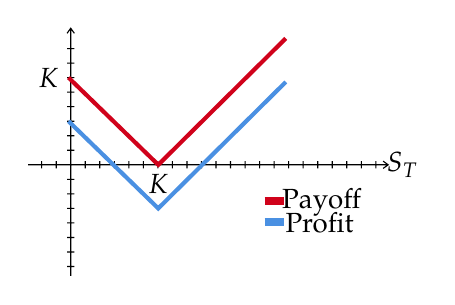
\begin{tikzpicture}[x=0.75pt,y=0.75pt,yscale=-0.35,xscale=0.35]
%uncomment if require: \path (0,363); %set diagram left start at 0, and has height of 363

%Shape: Axis 2D [id:dp04893296182422047] 
\draw  (14,196) -- (509.5,196)(72.5,8) -- (72.5,349) (502.5,191) -- (509.5,196) -- (502.5,201) (67.5,15) -- (72.5,8) -- (77.5,15) (92.5,191) -- (92.5,201)(112.5,191) -- (112.5,201)(132.5,191) -- (132.5,201)(152.5,191) -- (152.5,201)(172.5,191) -- (172.5,201)(192.5,191) -- (192.5,201)(212.5,191) -- (212.5,201)(232.5,191) -- (232.5,201)(252.5,191) -- (252.5,201)(272.5,191) -- (272.5,201)(292.5,191) -- (292.5,201)(312.5,191) -- (312.5,201)(332.5,191) -- (332.5,201)(352.5,191) -- (352.5,201)(372.5,191) -- (372.5,201)(392.5,191) -- (392.5,201)(412.5,191) -- (412.5,201)(432.5,191) -- (432.5,201)(452.5,191) -- (452.5,201)(472.5,191) -- (472.5,201)(492.5,191) -- (492.5,201)(52.5,191) -- (52.5,201)(32.5,191) -- (32.5,201)(67.5,176) -- (77.5,176)(67.5,156) -- (77.5,156)(67.5,136) -- (77.5,136)(67.5,116) -- (77.5,116)(67.5,96) -- (77.5,96)(67.5,76) -- (77.5,76)(67.5,56) -- (77.5,56)(67.5,36) -- (77.5,36)(67.5,216) -- (77.5,216)(67.5,236) -- (77.5,236)(67.5,256) -- (77.5,256)(67.5,276) -- (77.5,276)(67.5,296) -- (77.5,296)(67.5,316) -- (77.5,316)(67.5,336) -- (77.5,336) ;
\draw   ;
%Straight Lines [id:da29326132274692995] 
\draw [color={rgb, 255:red, 208; green, 2; blue, 27 }  ,draw opacity=1 ][line width=3]    (339.5,246) -- (366.5,246) ;


%Straight Lines [id:da0682309073045051] 
\draw [color={rgb, 255:red, 74; green, 144; blue, 226 }  ,draw opacity=1 ][line width=3]    (339.5,275) -- (366.5,275) ;



%Straight Lines [id:da6416016306991924] 
\draw [color={rgb, 255:red, 208; green, 2; blue, 27 }  ,draw opacity=1 ][line width=1.5]    (69.5,76) -- (193,196) -- (368.5,22) ;


%Straight Lines [id:da08174726568750468] 
\draw [color={rgb, 255:red, 74; green, 144; blue, 226 }  ,draw opacity=1 ][line width=1.5]    (69.5,136) -- (193,256) -- (368.5,82) ;



% Text Node
\draw (529,196) node  [align=left] {$\displaystyle S_{T}$};
% Text Node
\draw (418,247) node  [align=left] {Payoff};
% Text Node
\draw (415,276) node  [align=left] {Profit};
% Text Node
\draw (193,223) node   {$K$};
% Text Node
\draw (42,76) node   {$K$};


\end{tikzpicture}



\subsection*{Strangle}
Même genre de stratégie que le strangle, on spécule sur la volatilité du sous-jacent à l'extérieur de l'intervalle $[K_1, K_2]$ : 
\begin{align*}
Strangle			& = Put(K_1, T) + Call(K_2, T) \\
Premium			& = P(K_1, T) + C(K_2, T) > 0 \\
Payoff				& = 
\begin{cases}
K_1 - S_T			& , S_T \leq K_1 \\
0						& , K_1 < S_T \leq K_2 \\
S_T - K_2 		& , S_T > K_2 \\
\end{cases}
\end{align*}


\tikzset{every picture/.style={line width=0.75pt}} %set default line width to 0.75pt        

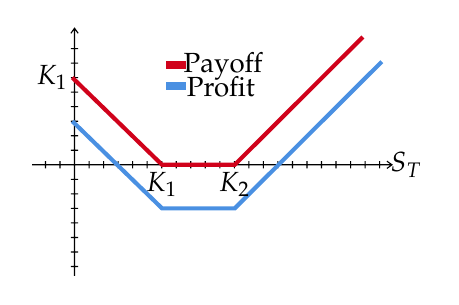
\begin{tikzpicture}[x=0.75pt,y=0.75pt,yscale=-0.35,xscale=0.35]
%uncomment if require: \path (0,363); %set diagram left start at 0, and has height of 363

%Shape: Axis 2D [id:dp20173159090508463] 
\draw  (14,196) -- (509.5,196)(72.5,8) -- (72.5,349) (502.5,191) -- (509.5,196) -- (502.5,201) (67.5,15) -- (72.5,8) -- (77.5,15) (92.5,191) -- (92.5,201)(112.5,191) -- (112.5,201)(132.5,191) -- (132.5,201)(152.5,191) -- (152.5,201)(172.5,191) -- (172.5,201)(192.5,191) -- (192.5,201)(212.5,191) -- (212.5,201)(232.5,191) -- (232.5,201)(252.5,191) -- (252.5,201)(272.5,191) -- (272.5,201)(292.5,191) -- (292.5,201)(312.5,191) -- (312.5,201)(332.5,191) -- (332.5,201)(352.5,191) -- (352.5,201)(372.5,191) -- (372.5,201)(392.5,191) -- (392.5,201)(412.5,191) -- (412.5,201)(432.5,191) -- (432.5,201)(452.5,191) -- (452.5,201)(472.5,191) -- (472.5,201)(492.5,191) -- (492.5,201)(52.5,191) -- (52.5,201)(32.5,191) -- (32.5,201)(67.5,176) -- (77.5,176)(67.5,156) -- (77.5,156)(67.5,136) -- (77.5,136)(67.5,116) -- (77.5,116)(67.5,96) -- (77.5,96)(67.5,76) -- (77.5,76)(67.5,56) -- (77.5,56)(67.5,36) -- (77.5,36)(67.5,216) -- (77.5,216)(67.5,236) -- (77.5,236)(67.5,256) -- (77.5,256)(67.5,276) -- (77.5,276)(67.5,296) -- (77.5,296)(67.5,316) -- (77.5,316)(67.5,336) -- (77.5,336) ;
\draw   ;
%Straight Lines [id:da06729302961101102] 
\draw [color={rgb, 255:red, 208; green, 2; blue, 27 }  ,draw opacity=1 ][line width=3]    (198.5,59) -- (225.5,59) ;


%Straight Lines [id:da7015689476766018] 
\draw [color={rgb, 255:red, 74; green, 144; blue, 226 }  ,draw opacity=1 ][line width=3]    (198.5,88) -- (225.5,88) ;



%Straight Lines [id:da5683323894945758] 
\draw [color={rgb, 255:red, 208; green, 2; blue, 27 }  ,draw opacity=1 ][line width=1.5]    (69.5,76) -- (193,196) -- (293,196) -- (469.5,20) ;


%Straight Lines [id:da06098365181250487] 
\draw [color={rgb, 255:red, 74; green, 144; blue, 226 }  ,draw opacity=1 ][line width=1.5]    (69.5,136) -- (193,256) -- (293,256) -- (495.5,54) ;



% Text Node
\draw (529,196) node  [align=left] {$\displaystyle S_{T}$};
% Text Node
\draw (277,60) node  [align=left] {Payoff};
% Text Node
\draw (274,89) node  [align=left] {Profit};
% Text Node
\draw (193,223) node   {$K_{1}$};
% Text Node
\draw (42,76) node   {$K_1$};
% Text Node
\draw (293,223) node   {$K_{2}$};


\end{tikzpicture}




\subsection*{Butterfly Spread (BFS)}
On combine un Straddle($K_2$) et un Strangle($K_1, K_3$) pour spéculer sur la non-volatilité du sous-jacent autour de $K_2$, mais en limitant nos pertes à $K_1 - K_2$ : 
\begin{align*}
Butterfly  & = Strangle - Straddle(K_2) \\
& = Put(K_1, T) - Put(K_2, T) \\
& - Call(K_2, T) + Call(K_3,T) \\
Premium	& = P(K_1, T) - P(K_2, T) \\
& - C(K_2, T) + C(K_3, T) < 0\\
Payoff		& = 
\begin{cases}
K_1 - K_2			& , S_T \leq K_1 \\
S_T - K_2			& , K_1 < S_T \leq K_2 \\
K_2 - S_T			& , K_2 < S_T \leq K_3 \\
K_2 - K_3			& , S_T > K_3 \\
\end{cases}
\end{align*}
\paragraph{Note} De façon générale (plusieurs combinaisons sont possibles), on a 
\[BFS = Bull(K_1, K_2) + Bear(K_2, K_3) \]


\tikzset{every picture/.style={line width=0.75pt}} %set default line width to 0.75pt        

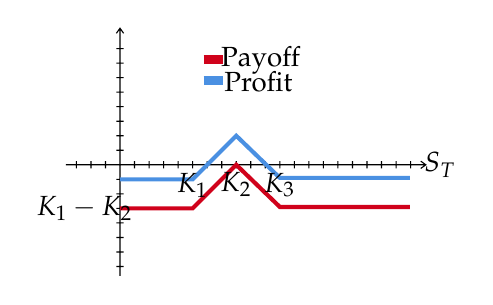
\begin{tikzpicture}[x=0.75pt,y=0.75pt,yscale=-0.35,xscale=0.35]
%uncomment if require: \path (0,363); %set diagram left start at 0, and has height of 363

%Shape: Axis 2D [id:dp516021239542077] 
\draw  (14,196) -- (509.5,196)(88.5,8) -- (88.5,349) (502.5,191) -- (509.5,196) -- (502.5,201) (83.5,15) -- (88.5,8) -- (93.5,15) (108.5,191) -- (108.5,201)(128.5,191) -- (128.5,201)(148.5,191) -- (148.5,201)(168.5,191) -- (168.5,201)(188.5,191) -- (188.5,201)(208.5,191) -- (208.5,201)(228.5,191) -- (228.5,201)(248.5,191) -- (248.5,201)(268.5,191) -- (268.5,201)(288.5,191) -- (288.5,201)(308.5,191) -- (308.5,201)(328.5,191) -- (328.5,201)(348.5,191) -- (348.5,201)(368.5,191) -- (368.5,201)(388.5,191) -- (388.5,201)(408.5,191) -- (408.5,201)(428.5,191) -- (428.5,201)(448.5,191) -- (448.5,201)(468.5,191) -- (468.5,201)(488.5,191) -- (488.5,201)(68.5,191) -- (68.5,201)(48.5,191) -- (48.5,201)(28.5,191) -- (28.5,201)(83.5,176) -- (93.5,176)(83.5,156) -- (93.5,156)(83.5,136) -- (93.5,136)(83.5,116) -- (93.5,116)(83.5,96) -- (93.5,96)(83.5,76) -- (93.5,76)(83.5,56) -- (93.5,56)(83.5,36) -- (93.5,36)(83.5,216) -- (93.5,216)(83.5,236) -- (93.5,236)(83.5,256) -- (93.5,256)(83.5,276) -- (93.5,276)(83.5,296) -- (93.5,296)(83.5,316) -- (93.5,316)(83.5,336) -- (93.5,336) ;
\draw   ;
%Straight Lines [id:da9881769874738698] 
\draw [color={rgb, 255:red, 208; green, 2; blue, 27 }  ,draw opacity=1 ][line width=3]    (203.5,51) -- (230.5,51) ;


%Straight Lines [id:da972554603165243] 
\draw [color={rgb, 255:red, 74; green, 144; blue, 226 }  ,draw opacity=1 ][line width=3]    (203.5,80) -- (230.5,80) ;



%Straight Lines [id:da5214606141485839] 
\draw [color={rgb, 255:red, 208; green, 2; blue, 27 }  ,draw opacity=1 ][line width=1.5]    (88.5,256) -- (188.5,256) -- (248.5,196) -- (308.5,254) -- (487.5,254) ;


%Straight Lines [id:da6207165128721853] 
\draw [color={rgb, 255:red, 74; green, 144; blue, 226 }  ,draw opacity=1 ][line width=1.5]    (88.5,216) -- (188.5,216) -- (248.5,156) -- (308.5,214) -- (487.5,214) ;



% Text Node
\draw (529,196) node  [align=left] {$\displaystyle S_{T}$};
% Text Node
\draw (282,52) node  [align=left] {Payoff};
% Text Node
\draw (279,81) node  [align=left] {Profit};
% Text Node
\draw (188.5,224) node   {$K_{1}$};
% Text Node
\draw (308.5,224) node   {$K_{3}$};
% Text Node
\draw (248.5,223) node   {$K_{2}$};
% Text Node
\draw (40,256) node   {$K_{1} -K_{2}$};


\end{tikzpicture}



\paragraph{Asymetric Butterfly Spread} 
\begin{itemize}
\item Comme le Ratio Spread, il est possible de faire une stratégie sur mesure en achetant $n$ Bull Spread et en achetant $m$ Bear Spread en respectant les 3 prix d'exercices $K_1 < K_2 < K_3$.
\item Si on désire avoir un BFS qui a un profit nul pour $S_T < K_1$ et $S_T > K_3$, alors on trouve $n$ et $m$ tel que
\begin{align*}
\frac{n}{m} = \frac{K_3 - K_2}{K_2 - K_1}
\end{align*}
\end{itemize}

% --- Chapitre 5 ---
% J'ai rassemblé une partie de la matière du chap.5 dans le chapitre 9, étant donné qu'on répétait de l'information.
\setcounter{section}{4}
\section{Forwards et Futures}
\subsection*{Forward avec dividendes}
\paragraph{Définition de base}
\[C(K,T) - P(K,T) = S_0 - K(1+r_f)^{T}\]

\paragraph{Action qui verse des dividendes}
\begin{align*}
C(K,T) - P(K,T) 		& = S - \text{PV}(Div) - K(1 + r_f)^{T} \\
& = S_0 e^{-\delta T} - K e^{-rT}
\end{align*}
où $\delta$ est un taux de versement des dividendes continu. \\

De plus, on a
\begin{align*}
F_{0,T} & = F_{0,T}^{P} (1 + r_f)^{T} \\
& = (S_0 - \text{PV}(div))(1+r_f)^{T} \\
& = S_0 - \sum_{i=1}^{T} d_i (1+r_f)^{T-i} \\
& = S_0 e^{(r-\delta)T}
\end{align*}

\paragraph{Forward synthétique avec dividendes}
On suppose le réinvestissement des dividendes.
\begin{align*}
\text{Forward}_{\text{avec div.}} & = e^{-\delta T} Stock - (e^{-\delta T} \cdot S_0) Bond \\
Premium		& =  e^{-\delta T} S_0 - e^{-\delta T} S_0 = 0 \\
Payoff			& = S_T - S_0 e^{(r-\delta) T}
\end{align*}

\paragraph{Cash-and-carry}
Stratégie qui consiste  à créer un Forward synthétique et vendre un Forward (profit nul).


\subsection*{Calcul avec prime de risque et nuance}
\begin{itemize}
\item Certains sous-jacent ont une composante de risque non-négligeable. Or, on ne peut pas dire que $F_{0,T} = \esp{S_T}$. Toutefois,
\[F_{0,T} = \esp{S_T} e^{-(\alpha - r) T}\]
\end{itemize}
où $\alpha$ est la prime de risque 	qu'on enlève pour obtenir le prix du Forward, tel que
\[\alpha = \underbrace{r}_{\text{Taux sans risque}} + \underbrace{(\alpha - r)}_{\text{Prime de risque}}\]

\subsection*{Forward de devise}
\paragraph{Put-Call parity avec les devises}
\begin{description}
\item[DD] Devise locale
\item[DÉ] Device étrangère
\item[$x_0$] Taux de change $\frac{DD}{DÉ}$ actuel ($t=0$)
\item[$r_D$] Taux sans risque \underline{local}
\item[$r_{É}$] Taux sans risque étranger
\end{description}
Le prix Forward prépayé pour une unité de DÉ à $t =0$ (payé en DD) est
\[F_{0,T}^{P}  = x_0 \left(1 + r_{É} \right)^{-T} \]
Et le prix Forward (à $t = T$) pour une unité de DÉ est
\begin{align*}
F_{0,T} & = F_{0,T}^{P} \left(1+r_D \right)^{T} \\
& = x_0 \left(  \frac{1+r_D}{1+r_{É}}   \right)^{T}\\
&  = x_0 e^{(r_D - r_{É})T}
\end{align*}

\paragraph{Forward synthétique de devise}
\begin{itemize}
\item Emprunt de $x_0(1+r_{É})^{-T}$ DD au taux $r_D$
\item Convertir les DD en DÉ
\item Dépôt de $(1+r_{É})^{-T}$ DÉ (au taux $r_{É}$) de 0 à $T$.
\end{itemize}
Le payoff sera $x_t - x_0 \left(  \frac{1+r_D}{1+r_{É}}   \right)^{T}$.


\subsection*{Future}
Essentiellement la même chose qu'un Forward, à quelques différences près : 
\begin{itemize}
\item Surveillé et contrôlé par des instances officielles (aucun \textit{Over-the-counter})
\item S'applique sur certains types d'actifs définis seulement ;
\item liquise et efficient
\item nécessite un dépôt initial des 2 parties (le risque de défaut est minimisé)
\item Transaction continues (règlement avec l'intermédiaire de façon quotidienne)
\item Variation extrêmes dans les prix de Future sont limités (possibilité du \textit{circuit Breaker})
\end{itemize}

\paragraph{Fonctionnement}
\begin{enumerate}
\item L'intermédaire demande un dépôt initial (\textit{initial margin}), \textbf{souvent un \% de la valeur notionnelle}.
\item Ce dépôt est accumulé à un taux de rendement $i$ fixé par l'intermédiaire.
\item À chaque période de règlement, on calcule la marge en fonction du prix du Future : \\
$\text{Marge}_T = \text{Marge}_{t} \cdot (1+i)^{T-t} + \text{Variation totale}_{[t,T]}$
\item Si $\text{Marge}_t  < \text{Maintenance margin}$\footnote{Cette marge est souvent exprimée en \% de la marge initiale.}, on doit \textbf{ajouter des fonds à la marge pour revenir à la marge initiale.}
avec $t < T$
\end{enumerate}



% --- Chapitre 9 ---
\setcounter{section}{8}
\section{Put-Call Parity}
\begin{align*}
Call - Put = Stock - Bond
\end{align*}

\subsection*{Put-Call Parity avec devises}
\begin{description}
\item[$Call(x_0, K, T)$ : ] Option d'achat qui permet d'acheter 1 unité de DÉ pour K unité de DD à l'échéance $t = T$.
\item[$Put(x_0, K, T)$ : ] Option de vente qui permet d'acheter 1 unité de DÉ pour K unité de DD à l'échéance $t = T$.
\end{description}
Alors, on peut réécrire l'équation Put-Call Parity : 
\begin{align*}
Call(x_0, K,T) - Put(x_0, K, T) = x_0(1+r_{É})^{-T} - K(1+r_D)^{-T}
\end{align*}


\subsection*{Parité généralisée et option d'échange}
\begin{description}
\item[$Call(S_t, Q_t, T - t)$ : ] Option d'achat qui permet d'acheter le sous-jacent $S$ au prix du sous-jacent $Q$ au temps $t = T$.
\item[$Put(S_t, Q_t, T - t)$ : ] Option de vente qui permet de vendre le sous-jacent $S$ au prix du sous-jacent $Q$ au temps $t = T$.
\end{description}
On peut généraliser l'équation Put-Call Parity : 
\begin{align*}
C(S_t, Q_t, T - t) - P(S_t, Q_t, T-t) = F_{t,T}^{P}(S) - F_{t,T}^{P}(Q)
\end{align*}

\subsection*{Options sur devise}
\begin{align*}
Call_{DD}(x_0, K, T) & = K \cdot Put_{DD}\left( \frac{1}{x_0}, \frac{1}{K}, T \right) \\
& = K \cdot x_0 \cdot Put_{DÉ} \left( \frac{1}{x_0}, \frac{1}{K}, T \right) \\
\end{align*}


\subsection*{Comparaison de différentes options}
\paragraph{Option américaine vs européenne}
\begin{align*}
C_{amer}(K,T) & \geq C_{euro}(K,T) \\
P_{amer}(K,T) & \geq P_{euro}(K,T) \\
\end{align*}

\paragraph{Option d'achat américaine}
Bien qu'on puisse exercer l'option américaine au moment qu'on veut, il \underline{peut} être optimal d'exercer avant l'échéance seulement si
\begin{align*}
PV(div) > K \left(1 - (1+r_f)^{-(T-t)} \right)
\end{align*}
ou si
\begin{align*}
PV(div) > P(K, T-t) + K \left(1 - (1+r_f)^{-(T-t)} \right)
\end{align*}

\paragraph{Option de vente américaine}
Le moment optimal pour exercer le Put serait tout juste \textbf{après la date ex-dividende}.



\paragraph{Date d'expiration}
Pour $T_1 < T_2$,
\begin{align*}
C(K, T_1) & \leq C(K, T_2) \\ 
P(K, T_1) & \leq P(K, T_2)
\end{align*}


\paragraph{Prix d'exercice}
Les différentes conditions énumérées ci-bas doivent être respectées : 
\begin{tabbing}
\hspace{5cm}\=\kill
 $C(K,T) \geq S_0 - K$ \>  $ P(K,T) \geq K - S_0$ \\ 
  $C(K_1, T) > C(K_2, T)$ \> $P(K_1, T) < P(K_2, T)$ \\
 $C(K_1, T) - C(K_2, T) \leq K_2 - K_1$ \> $P(K_2, T) - P(K_1, T) \leq K_2 - K_1$ \\
 $\frac{C(K_1, T) - C(K_2, T)}{K_2 - K_1} \geq \frac{C(K_2, T) - C(K_3, T)}{K_3 - K_2}$ \>  $\frac{P(K_2, T) - P(K_1, T)}{K_2 - K_1} \geq \frac{P(K_3, T) - P(K_2, T)}{K_3 - K_2}$ \\
\end{tabbing}
Si le prix d'exercice est \textit{Constant en valeur actualisée}\footnote{i.e. $K_t = K(1+r_f)^{T}$.}, alors, avec $t < T$
\begin{align*}
C(K_t, t) & \leq C(K_T, T) \\
P(K_t, t) & \leq P(K_T, T) \\
\end{align*}

% --- Chapitre 10 ---
\section{Introduction au modèle binomial d'évaluation des options}
\subsection*{Probabilité neutre au risque}
\begin{itemize}
\item $U = uS$ est la valeur supérieure que peut prendre le sous-jacent $S$
\item $D = dS$ est la valeur inférieure que peut prendre le sous-jacent $S$
\item $p$ est la probabilité (Bernouilli) que le sous-jacent prenne la valeur $U$.
\item $C_u$, $C_d$, $P_u$ et $P_d$ sont les payoff d'un call (ou put) selon la valeur du sous-jacent après $h$ périodes.
\item $r$ et $\delta$ sont respectivement la force d'intérêt sans risque et le taux de dividende continu.
\end{itemize}
 Alors, la probabilité \textit{neutre au risque} est
\begin{align*}
p = \frac{e^{(r-\delta)h} - d}{u-d}
\end{align*}

\subsection*{Portefeuille réplicatif d'une option}
On peut reproduire une option (Call ou Put) avec la stratégie suivante  :
\[C = \Delta S + B\]
où $B$ et $\Delta S$ changent de signe selon si c'est un Call ou un Put. On peut obtenir la prime initiale (\textit{Premium}) et les composantes du portefeuille réplicatif avec
\begin{align*}
\Delta = e^{-\delta h} \left( \frac{C_u - C_d}{U - D} \right) =   e^{-\delta h} \left( \frac{C_u - C_d}{S(u -d)} \right)
\end{align*}
\begin{align*}
B = e^{-rh} \left( \frac{U \cdot C_d - D \cdot C_u}{U - D} \right) = e^{-rh} \left( \frac{u C_d - d C_u}{u-d} \right)
\end{align*}
\begin{align*}
\text{Premium} = \Delta S_0 + B
\end{align*}


\end{multicols*}

%% -----------------------------
%% Fin du document
%% -----------------------------
\end{document}
